\documentclass[twoside]{book}

% Packages required by doxygen
\usepackage{fixltx2e}
\usepackage{calc}
\usepackage{doxygen}
\usepackage[export]{adjustbox} % also loads graphicx
\usepackage{graphicx}
\usepackage[utf8]{inputenc}
\usepackage{makeidx}
\usepackage{multicol}
\usepackage{multirow}
\PassOptionsToPackage{warn}{textcomp}
\usepackage{textcomp}
\usepackage[nointegrals]{wasysym}
\usepackage[table]{xcolor}

% Font selection
\usepackage[T1]{fontenc}
\usepackage[scaled=.90]{helvet}
\usepackage{courier}
\usepackage{amssymb}
\usepackage{sectsty}
\renewcommand{\familydefault}{\sfdefault}
\allsectionsfont{%
  \fontseries{bc}\selectfont%
  \color{darkgray}%
}
\renewcommand{\DoxyLabelFont}{%
  \fontseries{bc}\selectfont%
  \color{darkgray}%
}
\newcommand{\+}{\discretionary{\mbox{\scriptsize$\hookleftarrow$}}{}{}}

% Page & text layout
\usepackage{geometry}
\geometry{%
  a4paper,%
  top=2.5cm,%
  bottom=2.5cm,%
  left=2.5cm,%
  right=2.5cm%
}
\tolerance=750
\hfuzz=15pt
\hbadness=750
\setlength{\emergencystretch}{15pt}
\setlength{\parindent}{0cm}
\setlength{\parskip}{0.2cm}
\makeatletter
\renewcommand{\paragraph}{%
  \@startsection{paragraph}{4}{0ex}{-1.0ex}{1.0ex}{%
    \normalfont\normalsize\bfseries\SS@parafont%
  }%
}
\renewcommand{\subparagraph}{%
  \@startsection{subparagraph}{5}{0ex}{-1.0ex}{1.0ex}{%
    \normalfont\normalsize\bfseries\SS@subparafont%
  }%
}
\makeatother

% Headers & footers
\usepackage{fancyhdr}
\pagestyle{fancyplain}
\fancyhead[LE]{\fancyplain{}{\bfseries\thepage}}
\fancyhead[CE]{\fancyplain{}{}}
\fancyhead[RE]{\fancyplain{}{\bfseries\leftmark}}
\fancyhead[LO]{\fancyplain{}{\bfseries\rightmark}}
\fancyhead[CO]{\fancyplain{}{}}
\fancyhead[RO]{\fancyplain{}{\bfseries\thepage}}
\fancyfoot[LE]{\fancyplain{}{}}
\fancyfoot[CE]{\fancyplain{}{}}
\fancyfoot[RE]{\fancyplain{}{\bfseries\scriptsize Generated on Thu Jun 11 2015 12\+:09\+:54 for F\+Menu by Doxygen }}
\fancyfoot[LO]{\fancyplain{}{\bfseries\scriptsize Generated on Thu Jun 11 2015 12\+:09\+:54 for F\+Menu by Doxygen }}
\fancyfoot[CO]{\fancyplain{}{}}
\fancyfoot[RO]{\fancyplain{}{}}
\renewcommand{\footrulewidth}{0.4pt}
\renewcommand{\chaptermark}[1]{%
  \markboth{#1}{}%
}
\renewcommand{\sectionmark}[1]{%
  \markright{\thesection\ #1}%
}

% Indices & bibliography
\usepackage{natbib}
\usepackage[titles]{tocloft}
\setcounter{tocdepth}{3}
\setcounter{secnumdepth}{5}
\makeindex

% Hyperlinks (required, but should be loaded last)
\usepackage{ifpdf}
\ifpdf
  \usepackage[pdftex,pagebackref=true]{hyperref}
\else
  \usepackage[ps2pdf,pagebackref=true]{hyperref}
\fi
\hypersetup{%
  colorlinks=true,%
  linkcolor=blue,%
  citecolor=blue,%
  unicode%
}

% Custom commands
\newcommand{\clearemptydoublepage}{%
  \newpage{\pagestyle{empty}\cleardoublepage}%
}


%===== C O N T E N T S =====

\begin{document}

% Titlepage & ToC
\hypersetup{pageanchor=false,
             bookmarks=true,
             bookmarksnumbered=true,
             pdfencoding=unicode
            }
\pagenumbering{roman}
\begin{titlepage}
\vspace*{7cm}
\begin{center}%
{\Large F\+Menu }\\
\vspace*{1cm}
{\large Generated by Doxygen 1.8.9.1}\\
\vspace*{0.5cm}
{\small Thu Jun 11 2015 12:09:54}\\
\end{center}
\end{titlepage}
\clearemptydoublepage
\tableofcontents
\clearemptydoublepage
\pagenumbering{arabic}
\hypersetup{pageanchor=true}

%--- Begin generated contents ---
\chapter{Hierarchical Index}
\section{Class Hierarchy}
This inheritance list is sorted roughly, but not completely, alphabetically\+:\begin{DoxyCompactList}
\item \contentsline{section}{F\+Menu\+Facade}{\pageref{classFMenuFacade}}{}
\item \contentsline{section}{F\+Visitor}{\pageref{classFVisitor}}{}
\begin{DoxyCompactList}
\item \contentsline{section}{Insert\+Visitor}{\pageref{classInsertVisitor}}{}
\begin{DoxyCompactList}
\item \contentsline{section}{Remove\+Visitor}{\pageref{classRemoveVisitor}}{}
\end{DoxyCompactList}
\item \contentsline{section}{Menu\+Name\+Visitor}{\pageref{classMenuNameVisitor}}{}
\item \contentsline{section}{Select\+Element\+Visitor}{\pageref{classSelectElementVisitor}}{}
\end{DoxyCompactList}
\item \contentsline{section}{Menu\+Element}{\pageref{classMenuElement}}{}
\begin{DoxyCompactList}
\item \contentsline{section}{Menu\+Multi\+Select}{\pageref{classMenuMultiSelect}}{}
\item \contentsline{section}{Menu\+Single\+Select}{\pageref{classMenuSingleSelect}}{}
\end{DoxyCompactList}
\end{DoxyCompactList}

\chapter{Class Index}
\section{Class List}
Here are the classes, structs, unions and interfaces with brief descriptions\+:\begin{DoxyCompactList}
\item\contentsline{section}{\hyperlink{classFMenuFacade}{F\+Menu\+Facade} }{\pageref{classFMenuFacade}}{}
\item\contentsline{section}{\hyperlink{classFVisitor}{F\+Visitor} }{\pageref{classFVisitor}}{}
\item\contentsline{section}{\hyperlink{classInsertVisitor}{Insert\+Visitor} }{\pageref{classInsertVisitor}}{}
\item\contentsline{section}{\hyperlink{classMenuElement}{Menu\+Element} }{\pageref{classMenuElement}}{}
\item\contentsline{section}{\hyperlink{classMenuMultiSelect}{Menu\+Multi\+Select} }{\pageref{classMenuMultiSelect}}{}
\item\contentsline{section}{\hyperlink{classMenuNameVisitor}{Menu\+Name\+Visitor} }{\pageref{classMenuNameVisitor}}{}
\item\contentsline{section}{\hyperlink{classMenuSingleSelect}{Menu\+Single\+Select} }{\pageref{classMenuSingleSelect}}{}
\item\contentsline{section}{\hyperlink{classRemoveVisitor}{Remove\+Visitor} }{\pageref{classRemoveVisitor}}{}
\item\contentsline{section}{\hyperlink{classSelectElementVisitor}{Select\+Element\+Visitor} }{\pageref{classSelectElementVisitor}}{}
\end{DoxyCompactList}

\chapter{File Index}
\section{File List}
Here is a list of all files with brief descriptions\+:\begin{DoxyCompactList}
\item\contentsline{section}{\hyperlink{FMenuFacade_8cpp}{F\+Menu\+Facade.\+cpp} }{\pageref{FMenuFacade_8cpp}}{}
\item\contentsline{section}{\hyperlink{FMenuFacade_8h}{F\+Menu\+Facade.\+h} }{\pageref{FMenuFacade_8h}}{}
\item\contentsline{section}{\hyperlink{FVisitor_8cpp}{F\+Visitor.\+cpp} }{\pageref{FVisitor_8cpp}}{}
\item\contentsline{section}{\hyperlink{FVisitor_8h}{F\+Visitor.\+h} }{\pageref{FVisitor_8h}}{}
\item\contentsline{section}{\hyperlink{InsertVisitor_8cpp}{Insert\+Visitor.\+cpp} }{\pageref{InsertVisitor_8cpp}}{}
\item\contentsline{section}{\hyperlink{InsertVisitor_8h}{Insert\+Visitor.\+h} }{\pageref{InsertVisitor_8h}}{}
\item\contentsline{section}{\hyperlink{main_8cpp}{main.\+cpp} }{\pageref{main_8cpp}}{}
\item\contentsline{section}{\hyperlink{MenuElement_8cpp}{Menu\+Element.\+cpp} }{\pageref{MenuElement_8cpp}}{}
\item\contentsline{section}{\hyperlink{MenuElement_8h}{Menu\+Element.\+h} }{\pageref{MenuElement_8h}}{}
\item\contentsline{section}{\hyperlink{MenuMultiSelect_8cpp}{Menu\+Multi\+Select.\+cpp} }{\pageref{MenuMultiSelect_8cpp}}{}
\item\contentsline{section}{\hyperlink{MenuMultiSelect_8h}{Menu\+Multi\+Select.\+h} }{\pageref{MenuMultiSelect_8h}}{}
\item\contentsline{section}{\hyperlink{MenuNameVisitor_8cpp}{Menu\+Name\+Visitor.\+cpp} }{\pageref{MenuNameVisitor_8cpp}}{}
\item\contentsline{section}{\hyperlink{MenuNameVisitor_8h}{Menu\+Name\+Visitor.\+h} }{\pageref{MenuNameVisitor_8h}}{}
\item\contentsline{section}{\hyperlink{MenuSingleSelect_8cpp}{Menu\+Single\+Select.\+cpp} }{\pageref{MenuSingleSelect_8cpp}}{}
\item\contentsline{section}{\hyperlink{MenuSingleSelect_8h}{Menu\+Single\+Select.\+h} }{\pageref{MenuSingleSelect_8h}}{}
\item\contentsline{section}{\hyperlink{RemoveVisitor_8cpp}{Remove\+Visitor.\+cpp} }{\pageref{RemoveVisitor_8cpp}}{}
\item\contentsline{section}{\hyperlink{RemoveVisitor_8h}{Remove\+Visitor.\+h} }{\pageref{RemoveVisitor_8h}}{}
\item\contentsline{section}{\hyperlink{SelectElementVisitor_8cpp}{Select\+Element\+Visitor.\+cpp} }{\pageref{SelectElementVisitor_8cpp}}{}
\item\contentsline{section}{\hyperlink{SelectElementVisitor_8h}{Select\+Element\+Visitor.\+h} }{\pageref{SelectElementVisitor_8h}}{}
\end{DoxyCompactList}

\chapter{Class Documentation}
\hypertarget{classFMenuFacade}{}\section{F\+Menu\+Facade Class Reference}
\label{classFMenuFacade}\index{F\+Menu\+Facade@{F\+Menu\+Facade}}


{\ttfamily \#include $<$F\+Menu\+Facade.\+h$>$}



Collaboration diagram for F\+Menu\+Facade\+:
\nopagebreak
\begin{figure}[H]
\begin{center}
\leavevmode
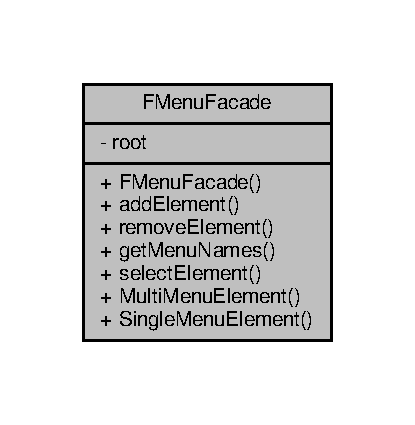
\includegraphics[width=199pt]{classFMenuFacade__coll__graph}
\end{center}
\end{figure}
\subsection*{Public Types}
\begin{DoxyCompactItemize}
\item 
typedef \hyperlink{classMenuNameVisitor_a8feb2ed73ab4a09c56a7f87ddd2d0478}{Menu\+Name\+Visitor\+::name\+\_\+list} \hyperlink{classFMenuFacade_a45d184d76216f6ce15b1b8b2fb4febb1}{name\+\_\+list}
\item 
typedef std\+::pair$<$ uint, std\+::string $>$ \hyperlink{classFMenuFacade_ad7061aee91a27742df50a0ee7c0201d2}{name}
\end{DoxyCompactItemize}
\subsection*{Public Member Functions}
\begin{DoxyCompactItemize}
\item 
\hyperlink{classFMenuFacade_acf26e00c686baac8da8b8f5e9eff3588}{F\+Menu\+Facade} (std\+::string \hyperlink{classFMenuFacade_ad7061aee91a27742df50a0ee7c0201d2}{name})
\item 
void \hyperlink{classFMenuFacade_a6f1b7f4b1ab3bf079fac28cca84445cc}{add\+Element} (uint pos, \hyperlink{classMenuElement}{Menu\+Element} $\ast$el)
\item 
void \hyperlink{classFMenuFacade_af371e6f6404b080c20e82e4355a0842e}{remove\+Element} (uint pos)
\item 
std\+::shared\+\_\+ptr$<$ \hyperlink{classFMenuFacade_a45d184d76216f6ce15b1b8b2fb4febb1}{name\+\_\+list} $>$ \hyperlink{classFMenuFacade_abc6dab5e91340476bc5eb7fcd3292095}{get\+Menu\+Names} ()
\item 
void \hyperlink{classFMenuFacade_a233201511b3316bcdeb2e772ef9a1700}{select\+Element} (uint pos)
\end{DoxyCompactItemize}
\subsection*{Static Public Member Functions}
\begin{DoxyCompactItemize}
\item 
static \hyperlink{classMenuElement}{Menu\+Element} $\ast$ \hyperlink{classFMenuFacade_a077a600d4fc54cbab61ffdfd4a4d0e8e}{Multi\+Menu\+Element} (std\+::string \hyperlink{classFMenuFacade_ad7061aee91a27742df50a0ee7c0201d2}{name})
\item 
static \hyperlink{classMenuElement}{Menu\+Element} $\ast$ \hyperlink{classFMenuFacade_afcf19a803927ea2fd6c86ad2576c7629}{Single\+Menu\+Element} (std\+::string \hyperlink{classFMenuFacade_ad7061aee91a27742df50a0ee7c0201d2}{name}, std\+::function$<$ void()$>$=\mbox{[}$\,$\mbox{]}\{\})
\end{DoxyCompactItemize}
\subsection*{Private Attributes}
\begin{DoxyCompactItemize}
\item 
std\+::unique\+\_\+ptr$<$ \hyperlink{classMenuMultiSelect}{Menu\+Multi\+Select} $>$ \hyperlink{classFMenuFacade_a00f246d05e03d88232a3b837584ab966}{root}
\end{DoxyCompactItemize}


\subsection{Member Typedef Documentation}
\hypertarget{classFMenuFacade_ad7061aee91a27742df50a0ee7c0201d2}{}\index{F\+Menu\+Facade@{F\+Menu\+Facade}!name@{name}}
\index{name@{name}!F\+Menu\+Facade@{F\+Menu\+Facade}}
\subsubsection[{name}]{\setlength{\rightskip}{0pt plus 5cm}typedef std\+::pair$<$uint, std\+::string$>$ {\bf F\+Menu\+Facade\+::name}}\label{classFMenuFacade_ad7061aee91a27742df50a0ee7c0201d2}
\hypertarget{classFMenuFacade_a45d184d76216f6ce15b1b8b2fb4febb1}{}\index{F\+Menu\+Facade@{F\+Menu\+Facade}!name\+\_\+list@{name\+\_\+list}}
\index{name\+\_\+list@{name\+\_\+list}!F\+Menu\+Facade@{F\+Menu\+Facade}}
\subsubsection[{name\+\_\+list}]{\setlength{\rightskip}{0pt plus 5cm}typedef {\bf Menu\+Name\+Visitor\+::name\+\_\+list} {\bf F\+Menu\+Facade\+::name\+\_\+list}}\label{classFMenuFacade_a45d184d76216f6ce15b1b8b2fb4febb1}


\subsection{Constructor \& Destructor Documentation}
\hypertarget{classFMenuFacade_acf26e00c686baac8da8b8f5e9eff3588}{}\index{F\+Menu\+Facade@{F\+Menu\+Facade}!F\+Menu\+Facade@{F\+Menu\+Facade}}
\index{F\+Menu\+Facade@{F\+Menu\+Facade}!F\+Menu\+Facade@{F\+Menu\+Facade}}
\subsubsection[{F\+Menu\+Facade}]{\setlength{\rightskip}{0pt plus 5cm}F\+Menu\+Facade\+::\+F\+Menu\+Facade (
\begin{DoxyParamCaption}
\item[{std\+::string}]{name}
\end{DoxyParamCaption}
)}\label{classFMenuFacade_acf26e00c686baac8da8b8f5e9eff3588}


\subsection{Member Function Documentation}
\hypertarget{classFMenuFacade_a6f1b7f4b1ab3bf079fac28cca84445cc}{}\index{F\+Menu\+Facade@{F\+Menu\+Facade}!add\+Element@{add\+Element}}
\index{add\+Element@{add\+Element}!F\+Menu\+Facade@{F\+Menu\+Facade}}
\subsubsection[{add\+Element}]{\setlength{\rightskip}{0pt plus 5cm}void F\+Menu\+Facade\+::add\+Element (
\begin{DoxyParamCaption}
\item[{uint}]{pos, }
\item[{{\bf Menu\+Element} $\ast$}]{el}
\end{DoxyParamCaption}
)}\label{classFMenuFacade_a6f1b7f4b1ab3bf079fac28cca84445cc}
\hypertarget{classFMenuFacade_abc6dab5e91340476bc5eb7fcd3292095}{}\index{F\+Menu\+Facade@{F\+Menu\+Facade}!get\+Menu\+Names@{get\+Menu\+Names}}
\index{get\+Menu\+Names@{get\+Menu\+Names}!F\+Menu\+Facade@{F\+Menu\+Facade}}
\subsubsection[{get\+Menu\+Names}]{\setlength{\rightskip}{0pt plus 5cm}std\+::shared\+\_\+ptr$<$ {\bf F\+Menu\+Facade\+::name\+\_\+list} $>$ F\+Menu\+Facade\+::get\+Menu\+Names (
\begin{DoxyParamCaption}
{}
\end{DoxyParamCaption}
)}\label{classFMenuFacade_abc6dab5e91340476bc5eb7fcd3292095}
\hypertarget{classFMenuFacade_a077a600d4fc54cbab61ffdfd4a4d0e8e}{}\index{F\+Menu\+Facade@{F\+Menu\+Facade}!Multi\+Menu\+Element@{Multi\+Menu\+Element}}
\index{Multi\+Menu\+Element@{Multi\+Menu\+Element}!F\+Menu\+Facade@{F\+Menu\+Facade}}
\subsubsection[{Multi\+Menu\+Element}]{\setlength{\rightskip}{0pt plus 5cm}{\bf Menu\+Element} $\ast$ F\+Menu\+Facade\+::\+Multi\+Menu\+Element (
\begin{DoxyParamCaption}
\item[{std\+::string}]{name}
\end{DoxyParamCaption}
)\hspace{0.3cm}{\ttfamily [static]}}\label{classFMenuFacade_a077a600d4fc54cbab61ffdfd4a4d0e8e}
\hypertarget{classFMenuFacade_af371e6f6404b080c20e82e4355a0842e}{}\index{F\+Menu\+Facade@{F\+Menu\+Facade}!remove\+Element@{remove\+Element}}
\index{remove\+Element@{remove\+Element}!F\+Menu\+Facade@{F\+Menu\+Facade}}
\subsubsection[{remove\+Element}]{\setlength{\rightskip}{0pt plus 5cm}void F\+Menu\+Facade\+::remove\+Element (
\begin{DoxyParamCaption}
\item[{uint}]{pos}
\end{DoxyParamCaption}
)}\label{classFMenuFacade_af371e6f6404b080c20e82e4355a0842e}
\hypertarget{classFMenuFacade_a233201511b3316bcdeb2e772ef9a1700}{}\index{F\+Menu\+Facade@{F\+Menu\+Facade}!select\+Element@{select\+Element}}
\index{select\+Element@{select\+Element}!F\+Menu\+Facade@{F\+Menu\+Facade}}
\subsubsection[{select\+Element}]{\setlength{\rightskip}{0pt plus 5cm}void F\+Menu\+Facade\+::select\+Element (
\begin{DoxyParamCaption}
\item[{uint}]{pos}
\end{DoxyParamCaption}
)}\label{classFMenuFacade_a233201511b3316bcdeb2e772ef9a1700}
\hypertarget{classFMenuFacade_afcf19a803927ea2fd6c86ad2576c7629}{}\index{F\+Menu\+Facade@{F\+Menu\+Facade}!Single\+Menu\+Element@{Single\+Menu\+Element}}
\index{Single\+Menu\+Element@{Single\+Menu\+Element}!F\+Menu\+Facade@{F\+Menu\+Facade}}
\subsubsection[{Single\+Menu\+Element}]{\setlength{\rightskip}{0pt plus 5cm}{\bf Menu\+Element} $\ast$ F\+Menu\+Facade\+::\+Single\+Menu\+Element (
\begin{DoxyParamCaption}
\item[{std\+::string}]{name, }
\item[{std\+::function$<$ void()$>$}]{function = {\ttfamily \mbox{[}\mbox{]}\{\}}}
\end{DoxyParamCaption}
)\hspace{0.3cm}{\ttfamily [static]}}\label{classFMenuFacade_afcf19a803927ea2fd6c86ad2576c7629}


\subsection{Member Data Documentation}
\hypertarget{classFMenuFacade_a00f246d05e03d88232a3b837584ab966}{}\index{F\+Menu\+Facade@{F\+Menu\+Facade}!root@{root}}
\index{root@{root}!F\+Menu\+Facade@{F\+Menu\+Facade}}
\subsubsection[{root}]{\setlength{\rightskip}{0pt plus 5cm}std\+::unique\+\_\+ptr$<${\bf Menu\+Multi\+Select}$>$ F\+Menu\+Facade\+::root\hspace{0.3cm}{\ttfamily [private]}}\label{classFMenuFacade_a00f246d05e03d88232a3b837584ab966}


The documentation for this class was generated from the following files\+:\begin{DoxyCompactItemize}
\item 
\hyperlink{FMenuFacade_8h}{F\+Menu\+Facade.\+h}\item 
\hyperlink{FMenuFacade_8cpp}{F\+Menu\+Facade.\+cpp}\end{DoxyCompactItemize}

\hypertarget{classFVisitor}{}\section{F\+Visitor Class Reference}
\label{classFVisitor}\index{F\+Visitor@{F\+Visitor}}


{\ttfamily \#include $<$F\+Visitor.\+h$>$}



Inheritance diagram for F\+Visitor\+:
\nopagebreak
\begin{figure}[H]
\begin{center}
\leavevmode
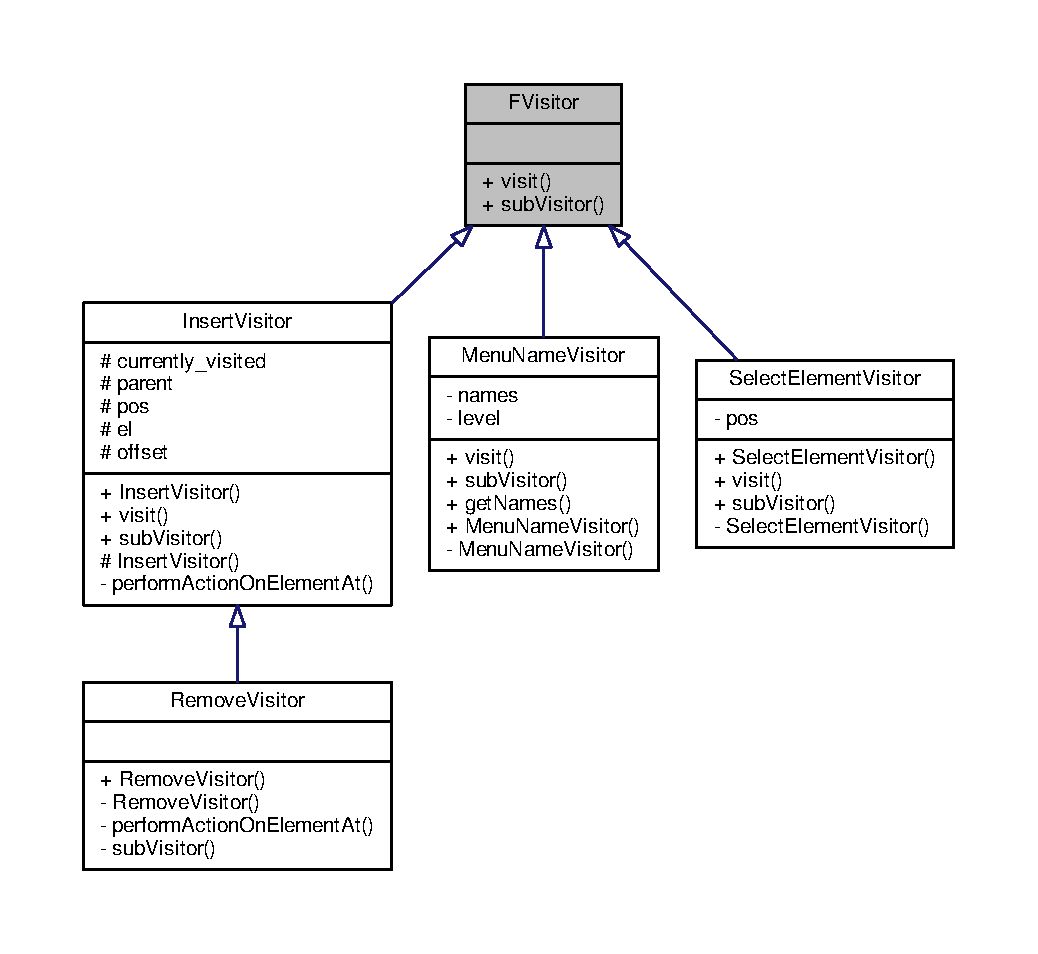
\includegraphics[width=350pt]{classFVisitor__inherit__graph}
\end{center}
\end{figure}


Collaboration diagram for F\+Visitor\+:
\nopagebreak
\begin{figure}[H]
\begin{center}
\leavevmode
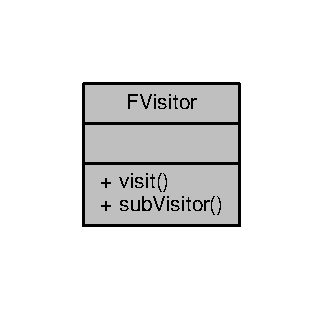
\includegraphics[width=155pt]{classFVisitor__coll__graph}
\end{center}
\end{figure}
\subsection*{Public Member Functions}
\begin{DoxyCompactItemize}
\item 
virtual void \hyperlink{classFVisitor_a42b99a5f7354fcd014eb44951d778058}{visit} (\hyperlink{classMenuElement}{Menu\+Element} $\ast$)=0
\item 
virtual std\+::unique\+\_\+ptr$<$ \hyperlink{classFVisitor}{F\+Visitor} $>$ \hyperlink{classFVisitor_ae7b318528ba0bd915a0c4958eb3fe437}{sub\+Visitor} ()=0
\end{DoxyCompactItemize}


\subsection{Member Function Documentation}
\hypertarget{classFVisitor_ae7b318528ba0bd915a0c4958eb3fe437}{}\index{F\+Visitor@{F\+Visitor}!sub\+Visitor@{sub\+Visitor}}
\index{sub\+Visitor@{sub\+Visitor}!F\+Visitor@{F\+Visitor}}
\subsubsection[{sub\+Visitor}]{\setlength{\rightskip}{0pt plus 5cm}virtual std\+::unique\+\_\+ptr$<${\bf F\+Visitor}$>$ F\+Visitor\+::sub\+Visitor (
\begin{DoxyParamCaption}
{}
\end{DoxyParamCaption}
)\hspace{0.3cm}{\ttfamily [pure virtual]}}\label{classFVisitor_ae7b318528ba0bd915a0c4958eb3fe437}


Implemented in \hyperlink{classRemoveVisitor_a44528eb89bc3150e3b322e367c1a7ffe}{Remove\+Visitor}, \hyperlink{classMenuNameVisitor_af766a058c692473485472ea569d5a54f}{Menu\+Name\+Visitor}, \hyperlink{classSelectElementVisitor_afa97120c24b6f67f81dfdb65bd243949}{Select\+Element\+Visitor}, and \hyperlink{classInsertVisitor_a6257a7684631f6ce7cf15855eb99c8f5}{Insert\+Visitor}.

\hypertarget{classFVisitor_a42b99a5f7354fcd014eb44951d778058}{}\index{F\+Visitor@{F\+Visitor}!visit@{visit}}
\index{visit@{visit}!F\+Visitor@{F\+Visitor}}
\subsubsection[{visit}]{\setlength{\rightskip}{0pt plus 5cm}virtual void F\+Visitor\+::visit (
\begin{DoxyParamCaption}
\item[{{\bf Menu\+Element} $\ast$}]{}
\end{DoxyParamCaption}
)\hspace{0.3cm}{\ttfamily [pure virtual]}}\label{classFVisitor_a42b99a5f7354fcd014eb44951d778058}


Implemented in \hyperlink{classMenuNameVisitor_a1289c718c9e60e329e68e6900c19be0f}{Menu\+Name\+Visitor}, \hyperlink{classInsertVisitor_a500b8f4ea580a84d0430b717ddd40d72}{Insert\+Visitor}, and \hyperlink{classSelectElementVisitor_af2dabf443aa6b32b253ca05baf3b780f}{Select\+Element\+Visitor}.



The documentation for this class was generated from the following file\+:\begin{DoxyCompactItemize}
\item 
\hyperlink{FVisitor_8h}{F\+Visitor.\+h}\end{DoxyCompactItemize}

\hypertarget{classInsertVisitor}{}\section{Insert\+Visitor Class Reference}
\label{classInsertVisitor}\index{Insert\+Visitor@{Insert\+Visitor}}


{\ttfamily \#include $<$Insert\+Visitor.\+h$>$}



Inheritance diagram for Insert\+Visitor\+:
\nopagebreak
\begin{figure}[H]
\begin{center}
\leavevmode
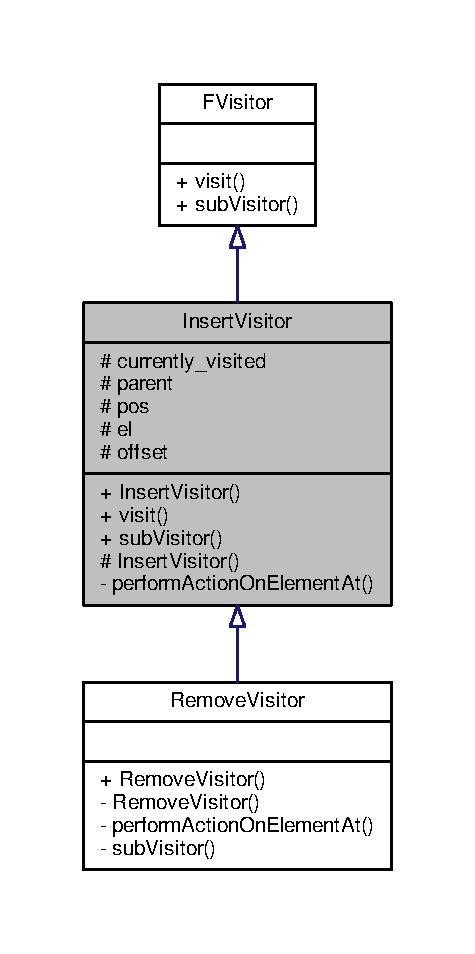
\includegraphics[width=228pt]{classInsertVisitor__inherit__graph}
\end{center}
\end{figure}


Collaboration diagram for Insert\+Visitor\+:
\nopagebreak
\begin{figure}[H]
\begin{center}
\leavevmode
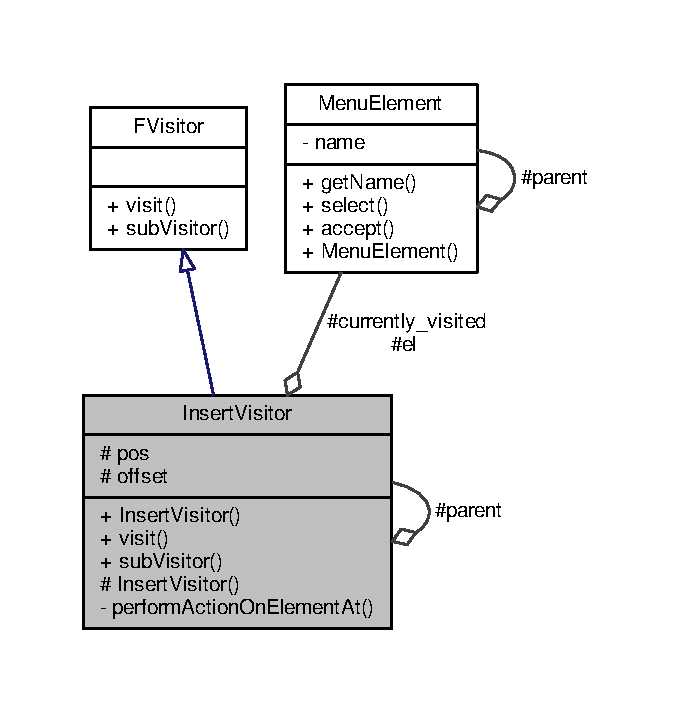
\includegraphics[width=323pt]{classInsertVisitor__coll__graph}
\end{center}
\end{figure}
\subsection*{Public Member Functions}
\begin{DoxyCompactItemize}
\item 
\hyperlink{classInsertVisitor_a33bed2522ab19248501fb405e3d02bff}{Insert\+Visitor} (\hyperlink{classMenuElement}{Menu\+Element} $\ast$\hyperlink{classInsertVisitor_a69e0d6193f75848df28ee23d538892fa}{el}, uint \hyperlink{classInsertVisitor_aeb7469f88fb024421c1dd9cfd3608d7d}{pos})
\item 
void \hyperlink{classInsertVisitor_a500b8f4ea580a84d0430b717ddd40d72}{visit} (\hyperlink{classMenuElement}{Menu\+Element} $\ast$) override
\item 
virtual std\+::unique\+\_\+ptr$<$ \hyperlink{classFVisitor}{F\+Visitor} $>$ \hyperlink{classInsertVisitor_a6257a7684631f6ce7cf15855eb99c8f5}{sub\+Visitor} () override
\end{DoxyCompactItemize}
\subsection*{Protected Member Functions}
\begin{DoxyCompactItemize}
\item 
\hyperlink{classInsertVisitor_afe0b93526e24543aef21ff47cd8cbbe9}{Insert\+Visitor} (\hyperlink{classMenuElement}{Menu\+Element} $\ast$\hyperlink{classInsertVisitor_a69e0d6193f75848df28ee23d538892fa}{el}, std\+::shared\+\_\+ptr$<$ uint $>$ \hyperlink{classInsertVisitor_aeb7469f88fb024421c1dd9cfd3608d7d}{pos}, \hyperlink{classInsertVisitor}{Insert\+Visitor} $\ast$\hyperlink{classInsertVisitor_a33db65fd081bd0448763274f1ca4632d}{parent})
\end{DoxyCompactItemize}
\subsection*{Protected Attributes}
\begin{DoxyCompactItemize}
\item 
\hyperlink{classMenuElement}{Menu\+Element} $\ast$ \hyperlink{classInsertVisitor_a12dabde0a05bc3909f2795a226c88053}{currently\+\_\+visited}
\item 
\hyperlink{classInsertVisitor}{Insert\+Visitor} $\ast$ \hyperlink{classInsertVisitor_a33db65fd081bd0448763274f1ca4632d}{parent}
\item 
std\+::shared\+\_\+ptr$<$ uint $>$ \hyperlink{classInsertVisitor_aeb7469f88fb024421c1dd9cfd3608d7d}{pos}
\item 
\hyperlink{classMenuElement}{Menu\+Element} $\ast$ \hyperlink{classInsertVisitor_a69e0d6193f75848df28ee23d538892fa}{el}
\item 
uint \hyperlink{classInsertVisitor_a46d57991e7305aff32cc2c8033986fc2}{offset}
\end{DoxyCompactItemize}
\subsection*{Private Member Functions}
\begin{DoxyCompactItemize}
\item 
virtual void \hyperlink{classInsertVisitor_a392e3ea0fd4f20801ce0d4e1a552d378}{perform\+Action\+On\+Element\+At} (uint \hyperlink{classInsertVisitor_a46d57991e7305aff32cc2c8033986fc2}{offset})
\end{DoxyCompactItemize}


\subsection{Constructor \& Destructor Documentation}
\hypertarget{classInsertVisitor_a33bed2522ab19248501fb405e3d02bff}{}\index{Insert\+Visitor@{Insert\+Visitor}!Insert\+Visitor@{Insert\+Visitor}}
\index{Insert\+Visitor@{Insert\+Visitor}!Insert\+Visitor@{Insert\+Visitor}}
\subsubsection[{Insert\+Visitor}]{\setlength{\rightskip}{0pt plus 5cm}Insert\+Visitor\+::\+Insert\+Visitor (
\begin{DoxyParamCaption}
\item[{{\bf Menu\+Element} $\ast$}]{el, }
\item[{uint}]{pos}
\end{DoxyParamCaption}
)\hspace{0.3cm}{\ttfamily [inline]}}\label{classInsertVisitor_a33bed2522ab19248501fb405e3d02bff}
\hypertarget{classInsertVisitor_afe0b93526e24543aef21ff47cd8cbbe9}{}\index{Insert\+Visitor@{Insert\+Visitor}!Insert\+Visitor@{Insert\+Visitor}}
\index{Insert\+Visitor@{Insert\+Visitor}!Insert\+Visitor@{Insert\+Visitor}}
\subsubsection[{Insert\+Visitor}]{\setlength{\rightskip}{0pt plus 5cm}Insert\+Visitor\+::\+Insert\+Visitor (
\begin{DoxyParamCaption}
\item[{{\bf Menu\+Element} $\ast$}]{el, }
\item[{std\+::shared\+\_\+ptr$<$ uint $>$}]{pos, }
\item[{{\bf Insert\+Visitor} $\ast$}]{parent}
\end{DoxyParamCaption}
)\hspace{0.3cm}{\ttfamily [inline]}, {\ttfamily [protected]}}\label{classInsertVisitor_afe0b93526e24543aef21ff47cd8cbbe9}


\subsection{Member Function Documentation}
\hypertarget{classInsertVisitor_a392e3ea0fd4f20801ce0d4e1a552d378}{}\index{Insert\+Visitor@{Insert\+Visitor}!perform\+Action\+On\+Element\+At@{perform\+Action\+On\+Element\+At}}
\index{perform\+Action\+On\+Element\+At@{perform\+Action\+On\+Element\+At}!Insert\+Visitor@{Insert\+Visitor}}
\subsubsection[{perform\+Action\+On\+Element\+At}]{\setlength{\rightskip}{0pt plus 5cm}void Insert\+Visitor\+::perform\+Action\+On\+Element\+At (
\begin{DoxyParamCaption}
\item[{uint}]{offset}
\end{DoxyParamCaption}
)\hspace{0.3cm}{\ttfamily [private]}, {\ttfamily [virtual]}}\label{classInsertVisitor_a392e3ea0fd4f20801ce0d4e1a552d378}


Reimplemented in \hyperlink{classRemoveVisitor_ae13ff6c08945e8e3e8d532d9cf905cfe}{Remove\+Visitor}.

\hypertarget{classInsertVisitor_a6257a7684631f6ce7cf15855eb99c8f5}{}\index{Insert\+Visitor@{Insert\+Visitor}!sub\+Visitor@{sub\+Visitor}}
\index{sub\+Visitor@{sub\+Visitor}!Insert\+Visitor@{Insert\+Visitor}}
\subsubsection[{sub\+Visitor}]{\setlength{\rightskip}{0pt plus 5cm}std\+::unique\+\_\+ptr$<$ {\bf F\+Visitor} $>$ Insert\+Visitor\+::sub\+Visitor (
\begin{DoxyParamCaption}
{}
\end{DoxyParamCaption}
)\hspace{0.3cm}{\ttfamily [override]}, {\ttfamily [virtual]}}\label{classInsertVisitor_a6257a7684631f6ce7cf15855eb99c8f5}


Implements \hyperlink{classFVisitor_ae7b318528ba0bd915a0c4958eb3fe437}{F\+Visitor}.



Reimplemented in \hyperlink{classRemoveVisitor_a44528eb89bc3150e3b322e367c1a7ffe}{Remove\+Visitor}.

\hypertarget{classInsertVisitor_a500b8f4ea580a84d0430b717ddd40d72}{}\index{Insert\+Visitor@{Insert\+Visitor}!visit@{visit}}
\index{visit@{visit}!Insert\+Visitor@{Insert\+Visitor}}
\subsubsection[{visit}]{\setlength{\rightskip}{0pt plus 5cm}void Insert\+Visitor\+::visit (
\begin{DoxyParamCaption}
\item[{{\bf Menu\+Element} $\ast$}]{el}
\end{DoxyParamCaption}
)\hspace{0.3cm}{\ttfamily [override]}, {\ttfamily [virtual]}}\label{classInsertVisitor_a500b8f4ea580a84d0430b717ddd40d72}


Implements \hyperlink{classFVisitor_a42b99a5f7354fcd014eb44951d778058}{F\+Visitor}.



\subsection{Member Data Documentation}
\hypertarget{classInsertVisitor_a12dabde0a05bc3909f2795a226c88053}{}\index{Insert\+Visitor@{Insert\+Visitor}!currently\+\_\+visited@{currently\+\_\+visited}}
\index{currently\+\_\+visited@{currently\+\_\+visited}!Insert\+Visitor@{Insert\+Visitor}}
\subsubsection[{currently\+\_\+visited}]{\setlength{\rightskip}{0pt plus 5cm}{\bf Menu\+Element}$\ast$ Insert\+Visitor\+::currently\+\_\+visited\hspace{0.3cm}{\ttfamily [protected]}}\label{classInsertVisitor_a12dabde0a05bc3909f2795a226c88053}
\hypertarget{classInsertVisitor_a69e0d6193f75848df28ee23d538892fa}{}\index{Insert\+Visitor@{Insert\+Visitor}!el@{el}}
\index{el@{el}!Insert\+Visitor@{Insert\+Visitor}}
\subsubsection[{el}]{\setlength{\rightskip}{0pt plus 5cm}{\bf Menu\+Element}$\ast$ Insert\+Visitor\+::el\hspace{0.3cm}{\ttfamily [protected]}}\label{classInsertVisitor_a69e0d6193f75848df28ee23d538892fa}
\hypertarget{classInsertVisitor_a46d57991e7305aff32cc2c8033986fc2}{}\index{Insert\+Visitor@{Insert\+Visitor}!offset@{offset}}
\index{offset@{offset}!Insert\+Visitor@{Insert\+Visitor}}
\subsubsection[{offset}]{\setlength{\rightskip}{0pt plus 5cm}uint Insert\+Visitor\+::offset\hspace{0.3cm}{\ttfamily [protected]}}\label{classInsertVisitor_a46d57991e7305aff32cc2c8033986fc2}
\hypertarget{classInsertVisitor_a33db65fd081bd0448763274f1ca4632d}{}\index{Insert\+Visitor@{Insert\+Visitor}!parent@{parent}}
\index{parent@{parent}!Insert\+Visitor@{Insert\+Visitor}}
\subsubsection[{parent}]{\setlength{\rightskip}{0pt plus 5cm}{\bf Insert\+Visitor}$\ast$ Insert\+Visitor\+::parent\hspace{0.3cm}{\ttfamily [protected]}}\label{classInsertVisitor_a33db65fd081bd0448763274f1ca4632d}
\hypertarget{classInsertVisitor_aeb7469f88fb024421c1dd9cfd3608d7d}{}\index{Insert\+Visitor@{Insert\+Visitor}!pos@{pos}}
\index{pos@{pos}!Insert\+Visitor@{Insert\+Visitor}}
\subsubsection[{pos}]{\setlength{\rightskip}{0pt plus 5cm}std\+::shared\+\_\+ptr$<$uint$>$ Insert\+Visitor\+::pos\hspace{0.3cm}{\ttfamily [protected]}}\label{classInsertVisitor_aeb7469f88fb024421c1dd9cfd3608d7d}


The documentation for this class was generated from the following files\+:\begin{DoxyCompactItemize}
\item 
\hyperlink{InsertVisitor_8h}{Insert\+Visitor.\+h}\item 
\hyperlink{InsertVisitor_8cpp}{Insert\+Visitor.\+cpp}\end{DoxyCompactItemize}

\hypertarget{classMenuElement}{}\section{Menu\+Element Class Reference}
\label{classMenuElement}\index{Menu\+Element@{Menu\+Element}}


{\ttfamily \#include $<$Menu\+Element.\+h$>$}



Inheritance diagram for Menu\+Element\+:
\nopagebreak
\begin{figure}[H]
\begin{center}
\leavevmode
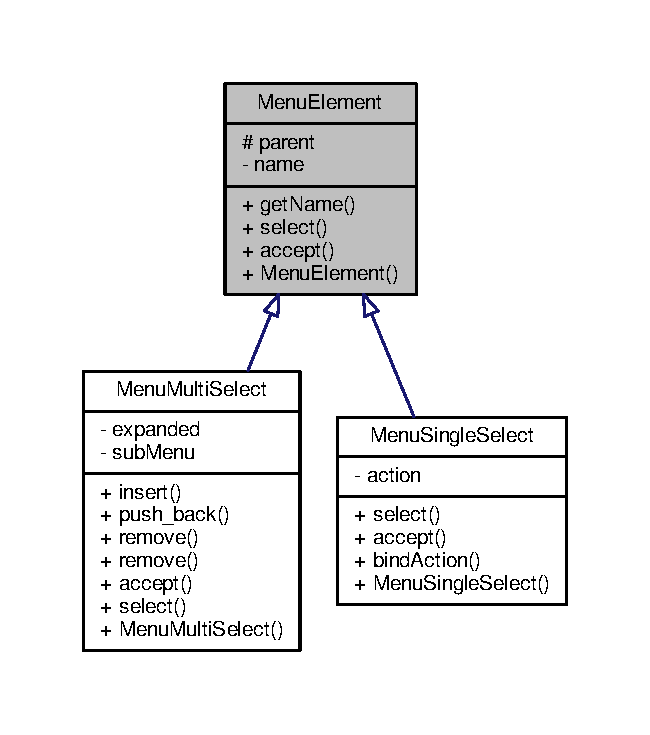
\includegraphics[width=312pt]{classMenuElement__inherit__graph}
\end{center}
\end{figure}


Collaboration diagram for Menu\+Element\+:
\nopagebreak
\begin{figure}[H]
\begin{center}
\leavevmode
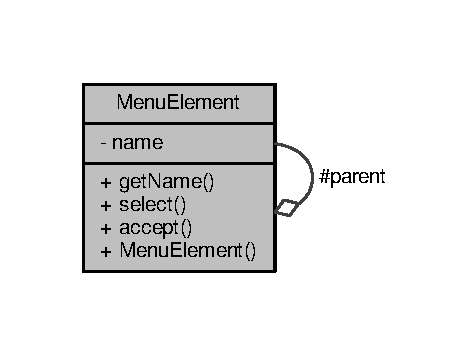
\includegraphics[width=226pt]{classMenuElement__coll__graph}
\end{center}
\end{figure}
\subsection*{Public Member Functions}
\begin{DoxyCompactItemize}
\item 
virtual std\+::string \hyperlink{classMenuElement_a70e00c3f10e97a04d1af14df4c50fe42}{get\+Name} () const 
\item 
virtual void \hyperlink{classMenuElement_afbe00cbf711c2b9e103131a66caca279}{select} ()=0
\item 
virtual void \hyperlink{classMenuElement_a98480beb81058617a721661517cb9c7f}{accept} (\hyperlink{classFVisitor}{F\+Visitor} \&, bool skip\+\_\+hidden=true)=0
\item 
\hyperlink{classMenuElement_a2620780bc0bc4abc3851eadd36a72b56}{Menu\+Element} (std\+::string \hyperlink{classMenuElement_ad7a280435eda4d231a68ae8645e7d98e}{name})
\end{DoxyCompactItemize}
\subsection*{Protected Attributes}
\begin{DoxyCompactItemize}
\item 
\hyperlink{classMenuElement}{Menu\+Element} $\ast$ \hyperlink{classMenuElement_a460f4e15826520bea44df1ef78f2b18f}{parent} = nullptr
\end{DoxyCompactItemize}
\subsection*{Private Attributes}
\begin{DoxyCompactItemize}
\item 
std\+::string \hyperlink{classMenuElement_ad7a280435eda4d231a68ae8645e7d98e}{name}
\end{DoxyCompactItemize}


\subsection{Constructor \& Destructor Documentation}
\hypertarget{classMenuElement_a2620780bc0bc4abc3851eadd36a72b56}{}\index{Menu\+Element@{Menu\+Element}!Menu\+Element@{Menu\+Element}}
\index{Menu\+Element@{Menu\+Element}!Menu\+Element@{Menu\+Element}}
\subsubsection[{Menu\+Element}]{\setlength{\rightskip}{0pt plus 5cm}Menu\+Element\+::\+Menu\+Element (
\begin{DoxyParamCaption}
\item[{std\+::string}]{name}
\end{DoxyParamCaption}
)\hspace{0.3cm}{\ttfamily [inline]}}\label{classMenuElement_a2620780bc0bc4abc3851eadd36a72b56}


\subsection{Member Function Documentation}
\hypertarget{classMenuElement_a98480beb81058617a721661517cb9c7f}{}\index{Menu\+Element@{Menu\+Element}!accept@{accept}}
\index{accept@{accept}!Menu\+Element@{Menu\+Element}}
\subsubsection[{accept}]{\setlength{\rightskip}{0pt plus 5cm}virtual void Menu\+Element\+::accept (
\begin{DoxyParamCaption}
\item[{{\bf F\+Visitor} \&}]{, }
\item[{bool}]{skip\+\_\+hidden = {\ttfamily true}}
\end{DoxyParamCaption}
)\hspace{0.3cm}{\ttfamily [pure virtual]}}\label{classMenuElement_a98480beb81058617a721661517cb9c7f}


Implemented in \hyperlink{classMenuMultiSelect_a0758f4d20b850ebe3562bfde651cf0bf}{Menu\+Multi\+Select}, and \hyperlink{classMenuSingleSelect_a58b681ca44f7f195a443e24c9c1fbb0f}{Menu\+Single\+Select}.

\hypertarget{classMenuElement_a70e00c3f10e97a04d1af14df4c50fe42}{}\index{Menu\+Element@{Menu\+Element}!get\+Name@{get\+Name}}
\index{get\+Name@{get\+Name}!Menu\+Element@{Menu\+Element}}
\subsubsection[{get\+Name}]{\setlength{\rightskip}{0pt plus 5cm}std\+::string Menu\+Element\+::get\+Name (
\begin{DoxyParamCaption}
{}
\end{DoxyParamCaption}
) const\hspace{0.3cm}{\ttfamily [virtual]}}\label{classMenuElement_a70e00c3f10e97a04d1af14df4c50fe42}
\hypertarget{classMenuElement_afbe00cbf711c2b9e103131a66caca279}{}\index{Menu\+Element@{Menu\+Element}!select@{select}}
\index{select@{select}!Menu\+Element@{Menu\+Element}}
\subsubsection[{select}]{\setlength{\rightskip}{0pt plus 5cm}virtual void Menu\+Element\+::select (
\begin{DoxyParamCaption}
{}
\end{DoxyParamCaption}
)\hspace{0.3cm}{\ttfamily [pure virtual]}}\label{classMenuElement_afbe00cbf711c2b9e103131a66caca279}


Implemented in \hyperlink{classMenuMultiSelect_a1f38785618e99e3644b5903811748be1}{Menu\+Multi\+Select}, and \hyperlink{classMenuSingleSelect_a1fdb45b9443e2e715665205cb383432b}{Menu\+Single\+Select}.



\subsection{Member Data Documentation}
\hypertarget{classMenuElement_ad7a280435eda4d231a68ae8645e7d98e}{}\index{Menu\+Element@{Menu\+Element}!name@{name}}
\index{name@{name}!Menu\+Element@{Menu\+Element}}
\subsubsection[{name}]{\setlength{\rightskip}{0pt plus 5cm}std\+::string Menu\+Element\+::name\hspace{0.3cm}{\ttfamily [private]}}\label{classMenuElement_ad7a280435eda4d231a68ae8645e7d98e}
\hypertarget{classMenuElement_a460f4e15826520bea44df1ef78f2b18f}{}\index{Menu\+Element@{Menu\+Element}!parent@{parent}}
\index{parent@{parent}!Menu\+Element@{Menu\+Element}}
\subsubsection[{parent}]{\setlength{\rightskip}{0pt plus 5cm}{\bf Menu\+Element}$\ast$ Menu\+Element\+::parent = nullptr\hspace{0.3cm}{\ttfamily [protected]}}\label{classMenuElement_a460f4e15826520bea44df1ef78f2b18f}


The documentation for this class was generated from the following files\+:\begin{DoxyCompactItemize}
\item 
\hyperlink{MenuElement_8h}{Menu\+Element.\+h}\item 
\hyperlink{MenuElement_8cpp}{Menu\+Element.\+cpp}\end{DoxyCompactItemize}

\hypertarget{classMenuMultiSelect}{}\section{Menu\+Multi\+Select Class Reference}
\label{classMenuMultiSelect}\index{Menu\+Multi\+Select@{Menu\+Multi\+Select}}


{\ttfamily \#include $<$Menu\+Multi\+Select.\+h$>$}



Inheritance diagram for Menu\+Multi\+Select\+:
\nopagebreak
\begin{figure}[H]
\begin{center}
\leavevmode
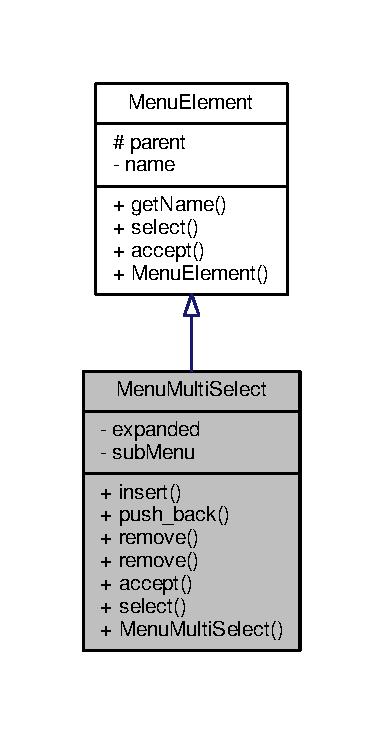
\includegraphics[width=184pt]{classMenuMultiSelect__inherit__graph}
\end{center}
\end{figure}


Collaboration diagram for Menu\+Multi\+Select\+:
\nopagebreak
\begin{figure}[H]
\begin{center}
\leavevmode
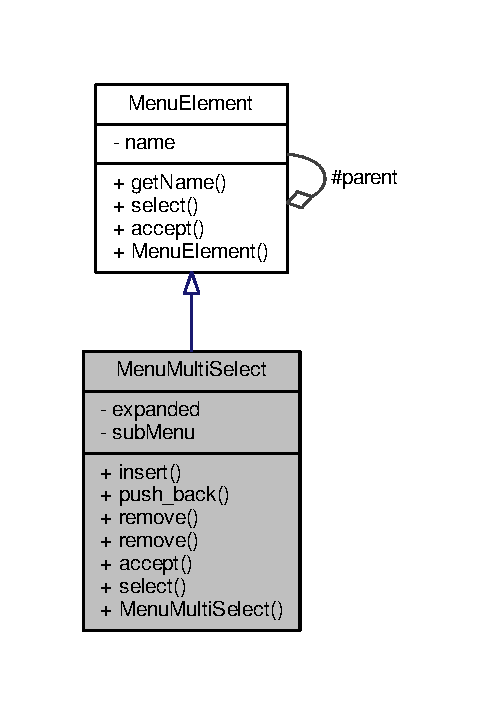
\includegraphics[width=232pt]{classMenuMultiSelect__coll__graph}
\end{center}
\end{figure}
\subsection*{Public Member Functions}
\begin{DoxyCompactItemize}
\item 
void \hyperlink{classMenuMultiSelect_af1b3f6f62c5bab3a4a461ac4a032fcc4}{insert} (uint pos, \hyperlink{classMenuElement}{Menu\+Element} $\ast$e)
\item 
void \hyperlink{classMenuMultiSelect_a56e4cbb5c191f0790a586ec36ffe0e0a}{push\+\_\+back} (\hyperlink{classMenuElement}{Menu\+Element} \&e)
\item 
void \hyperlink{classMenuMultiSelect_a0a96589db24c6ca38e582ab420a6f3db}{remove} (\hyperlink{classMenuElement}{Menu\+Element} $\ast$el)
\item 
void \hyperlink{classMenuMultiSelect_a22463f3a2494e9b465047bb02e768bc1}{remove} (uint pos)
\item 
void \hyperlink{classMenuMultiSelect_a0758f4d20b850ebe3562bfde651cf0bf}{accept} (\hyperlink{classFVisitor}{F\+Visitor} \&visitor, bool skip\+\_\+hidden=true) override
\item 
void \hyperlink{classMenuMultiSelect_a1f38785618e99e3644b5903811748be1}{select} () override
\item 
\hyperlink{classMenuMultiSelect_ac1f71e63de20e2ca46bccdf76d558068}{Menu\+Multi\+Select} (const std\+::string \&\hyperlink{classMenuElement_ad7a280435eda4d231a68ae8645e7d98e}{name})
\end{DoxyCompactItemize}
\subsection*{Private Attributes}
\begin{DoxyCompactItemize}
\item 
bool \hyperlink{classMenuMultiSelect_ac34317681355d1c48ef9ea003a2c35d8}{expanded} = true
\item 
std\+::vector$<$ std\+::unique\+\_\+ptr$<$ \hyperlink{classMenuElement}{Menu\+Element} $>$ $>$ \hyperlink{classMenuMultiSelect_a38d86e6f06968a8eaa2c4e215c95000a}{sub\+Menu}
\end{DoxyCompactItemize}
\subsection*{Additional Inherited Members}


\subsection{Constructor \& Destructor Documentation}
\hypertarget{classMenuMultiSelect_ac1f71e63de20e2ca46bccdf76d558068}{}\index{Menu\+Multi\+Select@{Menu\+Multi\+Select}!Menu\+Multi\+Select@{Menu\+Multi\+Select}}
\index{Menu\+Multi\+Select@{Menu\+Multi\+Select}!Menu\+Multi\+Select@{Menu\+Multi\+Select}}
\subsubsection[{Menu\+Multi\+Select}]{\setlength{\rightskip}{0pt plus 5cm}Menu\+Multi\+Select\+::\+Menu\+Multi\+Select (
\begin{DoxyParamCaption}
\item[{const std\+::string \&}]{name}
\end{DoxyParamCaption}
)\hspace{0.3cm}{\ttfamily [inline]}}\label{classMenuMultiSelect_ac1f71e63de20e2ca46bccdf76d558068}


\subsection{Member Function Documentation}
\hypertarget{classMenuMultiSelect_a0758f4d20b850ebe3562bfde651cf0bf}{}\index{Menu\+Multi\+Select@{Menu\+Multi\+Select}!accept@{accept}}
\index{accept@{accept}!Menu\+Multi\+Select@{Menu\+Multi\+Select}}
\subsubsection[{accept}]{\setlength{\rightskip}{0pt plus 5cm}void Menu\+Multi\+Select\+::accept (
\begin{DoxyParamCaption}
\item[{{\bf F\+Visitor} \&}]{visitor, }
\item[{bool}]{skip\+\_\+hidden = {\ttfamily true}}
\end{DoxyParamCaption}
)\hspace{0.3cm}{\ttfamily [override]}, {\ttfamily [virtual]}}\label{classMenuMultiSelect_a0758f4d20b850ebe3562bfde651cf0bf}


Implements \hyperlink{classMenuElement_a98480beb81058617a721661517cb9c7f}{Menu\+Element}.

\hypertarget{classMenuMultiSelect_af1b3f6f62c5bab3a4a461ac4a032fcc4}{}\index{Menu\+Multi\+Select@{Menu\+Multi\+Select}!insert@{insert}}
\index{insert@{insert}!Menu\+Multi\+Select@{Menu\+Multi\+Select}}
\subsubsection[{insert}]{\setlength{\rightskip}{0pt plus 5cm}void Menu\+Multi\+Select\+::insert (
\begin{DoxyParamCaption}
\item[{uint}]{pos, }
\item[{{\bf Menu\+Element} $\ast$}]{e}
\end{DoxyParamCaption}
)}\label{classMenuMultiSelect_af1b3f6f62c5bab3a4a461ac4a032fcc4}
\hypertarget{classMenuMultiSelect_a56e4cbb5c191f0790a586ec36ffe0e0a}{}\index{Menu\+Multi\+Select@{Menu\+Multi\+Select}!push\+\_\+back@{push\+\_\+back}}
\index{push\+\_\+back@{push\+\_\+back}!Menu\+Multi\+Select@{Menu\+Multi\+Select}}
\subsubsection[{push\+\_\+back}]{\setlength{\rightskip}{0pt plus 5cm}void Menu\+Multi\+Select\+::push\+\_\+back (
\begin{DoxyParamCaption}
\item[{{\bf Menu\+Element} \&}]{e}
\end{DoxyParamCaption}
)}\label{classMenuMultiSelect_a56e4cbb5c191f0790a586ec36ffe0e0a}
\hypertarget{classMenuMultiSelect_a0a96589db24c6ca38e582ab420a6f3db}{}\index{Menu\+Multi\+Select@{Menu\+Multi\+Select}!remove@{remove}}
\index{remove@{remove}!Menu\+Multi\+Select@{Menu\+Multi\+Select}}
\subsubsection[{remove}]{\setlength{\rightskip}{0pt plus 5cm}void Menu\+Multi\+Select\+::remove (
\begin{DoxyParamCaption}
\item[{{\bf Menu\+Element} $\ast$}]{el}
\end{DoxyParamCaption}
)}\label{classMenuMultiSelect_a0a96589db24c6ca38e582ab420a6f3db}
\hypertarget{classMenuMultiSelect_a22463f3a2494e9b465047bb02e768bc1}{}\index{Menu\+Multi\+Select@{Menu\+Multi\+Select}!remove@{remove}}
\index{remove@{remove}!Menu\+Multi\+Select@{Menu\+Multi\+Select}}
\subsubsection[{remove}]{\setlength{\rightskip}{0pt plus 5cm}void Menu\+Multi\+Select\+::remove (
\begin{DoxyParamCaption}
\item[{uint}]{pos}
\end{DoxyParamCaption}
)}\label{classMenuMultiSelect_a22463f3a2494e9b465047bb02e768bc1}
\hypertarget{classMenuMultiSelect_a1f38785618e99e3644b5903811748be1}{}\index{Menu\+Multi\+Select@{Menu\+Multi\+Select}!select@{select}}
\index{select@{select}!Menu\+Multi\+Select@{Menu\+Multi\+Select}}
\subsubsection[{select}]{\setlength{\rightskip}{0pt plus 5cm}void Menu\+Multi\+Select\+::select (
\begin{DoxyParamCaption}
{}
\end{DoxyParamCaption}
)\hspace{0.3cm}{\ttfamily [override]}, {\ttfamily [virtual]}}\label{classMenuMultiSelect_a1f38785618e99e3644b5903811748be1}


Implements \hyperlink{classMenuElement_afbe00cbf711c2b9e103131a66caca279}{Menu\+Element}.



\subsection{Member Data Documentation}
\hypertarget{classMenuMultiSelect_ac34317681355d1c48ef9ea003a2c35d8}{}\index{Menu\+Multi\+Select@{Menu\+Multi\+Select}!expanded@{expanded}}
\index{expanded@{expanded}!Menu\+Multi\+Select@{Menu\+Multi\+Select}}
\subsubsection[{expanded}]{\setlength{\rightskip}{0pt plus 5cm}bool Menu\+Multi\+Select\+::expanded = true\hspace{0.3cm}{\ttfamily [private]}}\label{classMenuMultiSelect_ac34317681355d1c48ef9ea003a2c35d8}
\hypertarget{classMenuMultiSelect_a38d86e6f06968a8eaa2c4e215c95000a}{}\index{Menu\+Multi\+Select@{Menu\+Multi\+Select}!sub\+Menu@{sub\+Menu}}
\index{sub\+Menu@{sub\+Menu}!Menu\+Multi\+Select@{Menu\+Multi\+Select}}
\subsubsection[{sub\+Menu}]{\setlength{\rightskip}{0pt plus 5cm}std\+::vector$<$std\+::unique\+\_\+ptr$<${\bf Menu\+Element}$>$ $>$ Menu\+Multi\+Select\+::sub\+Menu\hspace{0.3cm}{\ttfamily [private]}}\label{classMenuMultiSelect_a38d86e6f06968a8eaa2c4e215c95000a}


The documentation for this class was generated from the following files\+:\begin{DoxyCompactItemize}
\item 
\hyperlink{MenuMultiSelect_8h}{Menu\+Multi\+Select.\+h}\item 
\hyperlink{MenuMultiSelect_8cpp}{Menu\+Multi\+Select.\+cpp}\end{DoxyCompactItemize}

\hypertarget{classMenuNameVisitor}{}\section{Menu\+Name\+Visitor Class Reference}
\label{classMenuNameVisitor}\index{Menu\+Name\+Visitor@{Menu\+Name\+Visitor}}


{\ttfamily \#include $<$Menu\+Name\+Visitor.\+h$>$}



Inheritance diagram for Menu\+Name\+Visitor\+:
\nopagebreak
\begin{figure}[H]
\begin{center}
\leavevmode
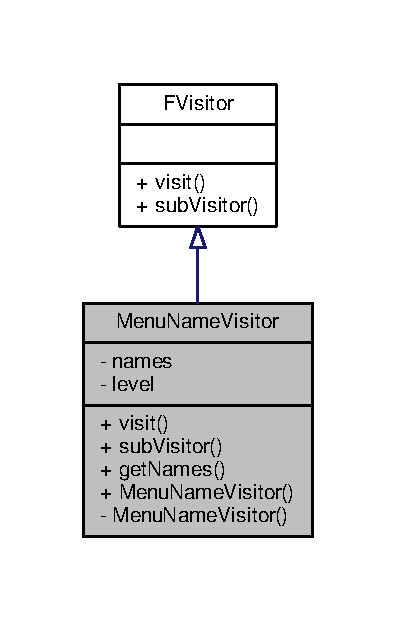
\includegraphics[width=190pt]{classMenuNameVisitor__inherit__graph}
\end{center}
\end{figure}


Collaboration diagram for Menu\+Name\+Visitor\+:
\nopagebreak
\begin{figure}[H]
\begin{center}
\leavevmode
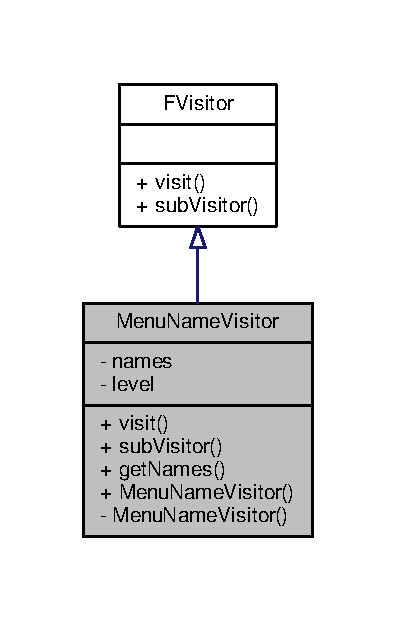
\includegraphics[width=190pt]{classMenuNameVisitor__coll__graph}
\end{center}
\end{figure}
\subsection*{Public Types}
\begin{DoxyCompactItemize}
\item 
typedef std\+::vector$<$ std\+::pair$<$ uint, std\+::string $>$ $>$ \hyperlink{classMenuNameVisitor_a8feb2ed73ab4a09c56a7f87ddd2d0478}{name\+\_\+list}
\item 
typedef std\+::pair$<$ uint, std\+::string $>$ \hyperlink{classMenuNameVisitor_a1ce6e7b626afbbcaa26785596900f531}{name}
\end{DoxyCompactItemize}
\subsection*{Public Member Functions}
\begin{DoxyCompactItemize}
\item 
virtual void \hyperlink{classMenuNameVisitor_a1289c718c9e60e329e68e6900c19be0f}{visit} (\hyperlink{classMenuElement}{Menu\+Element} $\ast$element) override
\item 
virtual std\+::unique\+\_\+ptr$<$ \hyperlink{classFVisitor}{F\+Visitor} $>$ \hyperlink{classMenuNameVisitor_af766a058c692473485472ea569d5a54f}{sub\+Visitor} () override
\item 
std\+::shared\+\_\+ptr$<$ \hyperlink{classMenuNameVisitor_a8feb2ed73ab4a09c56a7f87ddd2d0478}{name\+\_\+list} $>$ \hyperlink{classMenuNameVisitor_a9a8aead92197c2d1d63c5fa61b8f0b36}{get\+Names} ()
\item 
\hyperlink{classMenuNameVisitor_a17b31fe2e049705f3af50ecf9da00777}{Menu\+Name\+Visitor} ()
\end{DoxyCompactItemize}
\subsection*{Private Member Functions}
\begin{DoxyCompactItemize}
\item 
\hyperlink{classMenuNameVisitor_abba7f7e2b39a69a8ecc20eb570202e00}{Menu\+Name\+Visitor} (std\+::shared\+\_\+ptr$<$ \hyperlink{classMenuNameVisitor_a8feb2ed73ab4a09c56a7f87ddd2d0478}{name\+\_\+list} $>$ parent\+\_\+names, uint \hyperlink{classMenuNameVisitor_a77280f5654e700b95c1e22d32ae616fa}{level})
\end{DoxyCompactItemize}
\subsection*{Private Attributes}
\begin{DoxyCompactItemize}
\item 
std\+::shared\+\_\+ptr$<$ \hyperlink{classMenuNameVisitor_a8feb2ed73ab4a09c56a7f87ddd2d0478}{name\+\_\+list} $>$ \hyperlink{classMenuNameVisitor_a7237e6e9df65d870a95add62b07d1176}{names}
\item 
uint \hyperlink{classMenuNameVisitor_a77280f5654e700b95c1e22d32ae616fa}{level} = 0
\end{DoxyCompactItemize}


\subsection{Member Typedef Documentation}
\hypertarget{classMenuNameVisitor_a1ce6e7b626afbbcaa26785596900f531}{}\index{Menu\+Name\+Visitor@{Menu\+Name\+Visitor}!name@{name}}
\index{name@{name}!Menu\+Name\+Visitor@{Menu\+Name\+Visitor}}
\subsubsection[{name}]{\setlength{\rightskip}{0pt plus 5cm}typedef std\+::pair$<$uint, std\+::string$>$ {\bf Menu\+Name\+Visitor\+::name}}\label{classMenuNameVisitor_a1ce6e7b626afbbcaa26785596900f531}
\hypertarget{classMenuNameVisitor_a8feb2ed73ab4a09c56a7f87ddd2d0478}{}\index{Menu\+Name\+Visitor@{Menu\+Name\+Visitor}!name\+\_\+list@{name\+\_\+list}}
\index{name\+\_\+list@{name\+\_\+list}!Menu\+Name\+Visitor@{Menu\+Name\+Visitor}}
\subsubsection[{name\+\_\+list}]{\setlength{\rightskip}{0pt plus 5cm}typedef std\+::vector$<$std\+::pair$<$uint, std\+::string$>$ $>$ {\bf Menu\+Name\+Visitor\+::name\+\_\+list}}\label{classMenuNameVisitor_a8feb2ed73ab4a09c56a7f87ddd2d0478}


\subsection{Constructor \& Destructor Documentation}
\hypertarget{classMenuNameVisitor_a17b31fe2e049705f3af50ecf9da00777}{}\index{Menu\+Name\+Visitor@{Menu\+Name\+Visitor}!Menu\+Name\+Visitor@{Menu\+Name\+Visitor}}
\index{Menu\+Name\+Visitor@{Menu\+Name\+Visitor}!Menu\+Name\+Visitor@{Menu\+Name\+Visitor}}
\subsubsection[{Menu\+Name\+Visitor}]{\setlength{\rightskip}{0pt plus 5cm}Menu\+Name\+Visitor\+::\+Menu\+Name\+Visitor (
\begin{DoxyParamCaption}
{}
\end{DoxyParamCaption}
)}\label{classMenuNameVisitor_a17b31fe2e049705f3af50ecf9da00777}
\hypertarget{classMenuNameVisitor_abba7f7e2b39a69a8ecc20eb570202e00}{}\index{Menu\+Name\+Visitor@{Menu\+Name\+Visitor}!Menu\+Name\+Visitor@{Menu\+Name\+Visitor}}
\index{Menu\+Name\+Visitor@{Menu\+Name\+Visitor}!Menu\+Name\+Visitor@{Menu\+Name\+Visitor}}
\subsubsection[{Menu\+Name\+Visitor}]{\setlength{\rightskip}{0pt plus 5cm}Menu\+Name\+Visitor\+::\+Menu\+Name\+Visitor (
\begin{DoxyParamCaption}
\item[{std\+::shared\+\_\+ptr$<$ {\bf name\+\_\+list} $>$}]{parent\+\_\+names, }
\item[{uint}]{level}
\end{DoxyParamCaption}
)\hspace{0.3cm}{\ttfamily [private]}}\label{classMenuNameVisitor_abba7f7e2b39a69a8ecc20eb570202e00}


\subsection{Member Function Documentation}
\hypertarget{classMenuNameVisitor_a9a8aead92197c2d1d63c5fa61b8f0b36}{}\index{Menu\+Name\+Visitor@{Menu\+Name\+Visitor}!get\+Names@{get\+Names}}
\index{get\+Names@{get\+Names}!Menu\+Name\+Visitor@{Menu\+Name\+Visitor}}
\subsubsection[{get\+Names}]{\setlength{\rightskip}{0pt plus 5cm}std\+::shared\+\_\+ptr$<$ {\bf Menu\+Name\+Visitor\+::name\+\_\+list} $>$ Menu\+Name\+Visitor\+::get\+Names (
\begin{DoxyParamCaption}
{}
\end{DoxyParamCaption}
)}\label{classMenuNameVisitor_a9a8aead92197c2d1d63c5fa61b8f0b36}
\hypertarget{classMenuNameVisitor_af766a058c692473485472ea569d5a54f}{}\index{Menu\+Name\+Visitor@{Menu\+Name\+Visitor}!sub\+Visitor@{sub\+Visitor}}
\index{sub\+Visitor@{sub\+Visitor}!Menu\+Name\+Visitor@{Menu\+Name\+Visitor}}
\subsubsection[{sub\+Visitor}]{\setlength{\rightskip}{0pt plus 5cm}std\+::unique\+\_\+ptr$<$ {\bf F\+Visitor} $>$ Menu\+Name\+Visitor\+::sub\+Visitor (
\begin{DoxyParamCaption}
{}
\end{DoxyParamCaption}
)\hspace{0.3cm}{\ttfamily [override]}, {\ttfamily [virtual]}}\label{classMenuNameVisitor_af766a058c692473485472ea569d5a54f}


Implements \hyperlink{classFVisitor_ae7b318528ba0bd915a0c4958eb3fe437}{F\+Visitor}.

\hypertarget{classMenuNameVisitor_a1289c718c9e60e329e68e6900c19be0f}{}\index{Menu\+Name\+Visitor@{Menu\+Name\+Visitor}!visit@{visit}}
\index{visit@{visit}!Menu\+Name\+Visitor@{Menu\+Name\+Visitor}}
\subsubsection[{visit}]{\setlength{\rightskip}{0pt plus 5cm}void Menu\+Name\+Visitor\+::visit (
\begin{DoxyParamCaption}
\item[{{\bf Menu\+Element} $\ast$}]{element}
\end{DoxyParamCaption}
)\hspace{0.3cm}{\ttfamily [override]}, {\ttfamily [virtual]}}\label{classMenuNameVisitor_a1289c718c9e60e329e68e6900c19be0f}


Implements \hyperlink{classFVisitor_a42b99a5f7354fcd014eb44951d778058}{F\+Visitor}.



\subsection{Member Data Documentation}
\hypertarget{classMenuNameVisitor_a77280f5654e700b95c1e22d32ae616fa}{}\index{Menu\+Name\+Visitor@{Menu\+Name\+Visitor}!level@{level}}
\index{level@{level}!Menu\+Name\+Visitor@{Menu\+Name\+Visitor}}
\subsubsection[{level}]{\setlength{\rightskip}{0pt plus 5cm}uint Menu\+Name\+Visitor\+::level = 0\hspace{0.3cm}{\ttfamily [private]}}\label{classMenuNameVisitor_a77280f5654e700b95c1e22d32ae616fa}
\hypertarget{classMenuNameVisitor_a7237e6e9df65d870a95add62b07d1176}{}\index{Menu\+Name\+Visitor@{Menu\+Name\+Visitor}!names@{names}}
\index{names@{names}!Menu\+Name\+Visitor@{Menu\+Name\+Visitor}}
\subsubsection[{names}]{\setlength{\rightskip}{0pt plus 5cm}std\+::shared\+\_\+ptr$<${\bf name\+\_\+list}$>$ Menu\+Name\+Visitor\+::names\hspace{0.3cm}{\ttfamily [private]}}\label{classMenuNameVisitor_a7237e6e9df65d870a95add62b07d1176}


The documentation for this class was generated from the following files\+:\begin{DoxyCompactItemize}
\item 
\hyperlink{MenuNameVisitor_8h}{Menu\+Name\+Visitor.\+h}\item 
\hyperlink{MenuNameVisitor_8cpp}{Menu\+Name\+Visitor.\+cpp}\end{DoxyCompactItemize}

\hypertarget{classMenuSingleSelect}{}\section{Menu\+Single\+Select Class Reference}
\label{classMenuSingleSelect}\index{Menu\+Single\+Select@{Menu\+Single\+Select}}


{\ttfamily \#include $<$Menu\+Single\+Select.\+h$>$}



Inheritance diagram for Menu\+Single\+Select\+:
\nopagebreak
\begin{figure}[H]
\begin{center}
\leavevmode
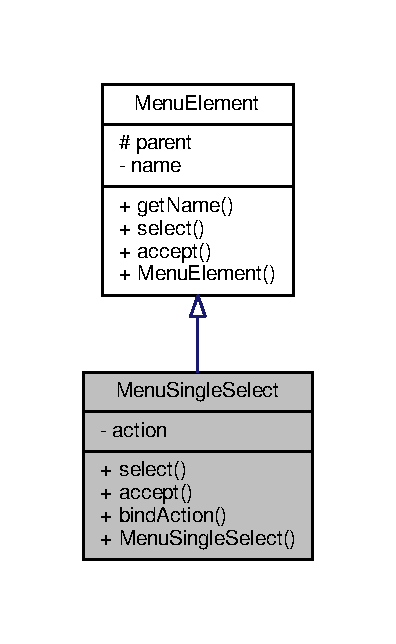
\includegraphics[width=190pt]{classMenuSingleSelect__inherit__graph}
\end{center}
\end{figure}


Collaboration diagram for Menu\+Single\+Select\+:
\nopagebreak
\begin{figure}[H]
\begin{center}
\leavevmode
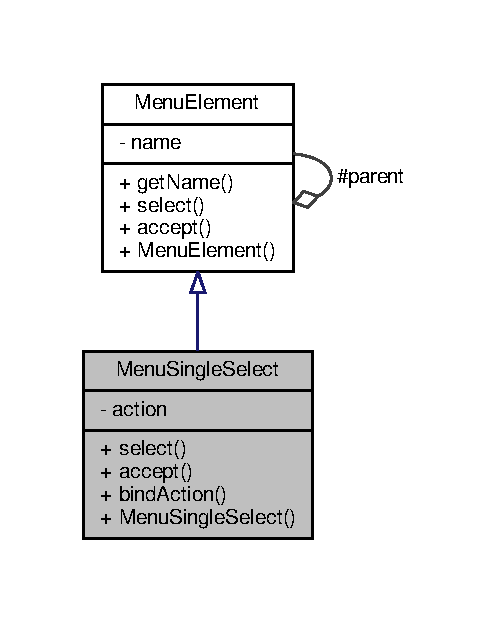
\includegraphics[width=235pt]{classMenuSingleSelect__coll__graph}
\end{center}
\end{figure}
\subsection*{Public Member Functions}
\begin{DoxyCompactItemize}
\item 
virtual void \hyperlink{classMenuSingleSelect_a1fdb45b9443e2e715665205cb383432b}{select} () override
\item 
virtual void \hyperlink{classMenuSingleSelect_a58b681ca44f7f195a443e24c9c1fbb0f}{accept} (\hyperlink{classFVisitor}{F\+Visitor} \&visitor, bool) override
\item 
virtual void \hyperlink{classMenuSingleSelect_a69ecc13765a7fd247f90fd7a231fb0e1}{bind\+Action} (std\+::function$<$ void()$>$ function)
\item 
\hyperlink{classMenuSingleSelect_a8e800f51a266863900f44be84f11b1ba}{Menu\+Single\+Select} (std\+::string \hyperlink{classMenuElement_ad7a280435eda4d231a68ae8645e7d98e}{name})
\end{DoxyCompactItemize}
\subsection*{Private Attributes}
\begin{DoxyCompactItemize}
\item 
std\+::function$<$ void()$>$ \hyperlink{classMenuSingleSelect_a6f6a86250fd0057b52eef71b78538e56}{action}
\end{DoxyCompactItemize}
\subsection*{Additional Inherited Members}


\subsection{Constructor \& Destructor Documentation}
\hypertarget{classMenuSingleSelect_a8e800f51a266863900f44be84f11b1ba}{}\index{Menu\+Single\+Select@{Menu\+Single\+Select}!Menu\+Single\+Select@{Menu\+Single\+Select}}
\index{Menu\+Single\+Select@{Menu\+Single\+Select}!Menu\+Single\+Select@{Menu\+Single\+Select}}
\subsubsection[{Menu\+Single\+Select}]{\setlength{\rightskip}{0pt plus 5cm}Menu\+Single\+Select\+::\+Menu\+Single\+Select (
\begin{DoxyParamCaption}
\item[{std\+::string}]{name}
\end{DoxyParamCaption}
)}\label{classMenuSingleSelect_a8e800f51a266863900f44be84f11b1ba}


\subsection{Member Function Documentation}
\hypertarget{classMenuSingleSelect_a58b681ca44f7f195a443e24c9c1fbb0f}{}\index{Menu\+Single\+Select@{Menu\+Single\+Select}!accept@{accept}}
\index{accept@{accept}!Menu\+Single\+Select@{Menu\+Single\+Select}}
\subsubsection[{accept}]{\setlength{\rightskip}{0pt plus 5cm}void Menu\+Single\+Select\+::accept (
\begin{DoxyParamCaption}
\item[{{\bf F\+Visitor} \&}]{visitor, }
\item[{bool}]{}
\end{DoxyParamCaption}
)\hspace{0.3cm}{\ttfamily [override]}, {\ttfamily [virtual]}}\label{classMenuSingleSelect_a58b681ca44f7f195a443e24c9c1fbb0f}


Implements \hyperlink{classMenuElement_a98480beb81058617a721661517cb9c7f}{Menu\+Element}.

\hypertarget{classMenuSingleSelect_a69ecc13765a7fd247f90fd7a231fb0e1}{}\index{Menu\+Single\+Select@{Menu\+Single\+Select}!bind\+Action@{bind\+Action}}
\index{bind\+Action@{bind\+Action}!Menu\+Single\+Select@{Menu\+Single\+Select}}
\subsubsection[{bind\+Action}]{\setlength{\rightskip}{0pt plus 5cm}void Menu\+Single\+Select\+::bind\+Action (
\begin{DoxyParamCaption}
\item[{std\+::function$<$ void()$>$}]{function}
\end{DoxyParamCaption}
)\hspace{0.3cm}{\ttfamily [virtual]}}\label{classMenuSingleSelect_a69ecc13765a7fd247f90fd7a231fb0e1}
\hypertarget{classMenuSingleSelect_a1fdb45b9443e2e715665205cb383432b}{}\index{Menu\+Single\+Select@{Menu\+Single\+Select}!select@{select}}
\index{select@{select}!Menu\+Single\+Select@{Menu\+Single\+Select}}
\subsubsection[{select}]{\setlength{\rightskip}{0pt plus 5cm}void Menu\+Single\+Select\+::select (
\begin{DoxyParamCaption}
{}
\end{DoxyParamCaption}
)\hspace{0.3cm}{\ttfamily [override]}, {\ttfamily [virtual]}}\label{classMenuSingleSelect_a1fdb45b9443e2e715665205cb383432b}


Implements \hyperlink{classMenuElement_afbe00cbf711c2b9e103131a66caca279}{Menu\+Element}.



\subsection{Member Data Documentation}
\hypertarget{classMenuSingleSelect_a6f6a86250fd0057b52eef71b78538e56}{}\index{Menu\+Single\+Select@{Menu\+Single\+Select}!action@{action}}
\index{action@{action}!Menu\+Single\+Select@{Menu\+Single\+Select}}
\subsubsection[{action}]{\setlength{\rightskip}{0pt plus 5cm}std\+::function$<$void()$>$ Menu\+Single\+Select\+::action\hspace{0.3cm}{\ttfamily [private]}}\label{classMenuSingleSelect_a6f6a86250fd0057b52eef71b78538e56}


The documentation for this class was generated from the following files\+:\begin{DoxyCompactItemize}
\item 
\hyperlink{MenuSingleSelect_8h}{Menu\+Single\+Select.\+h}\item 
\hyperlink{MenuSingleSelect_8cpp}{Menu\+Single\+Select.\+cpp}\end{DoxyCompactItemize}

\hypertarget{classRemoveVisitor}{}\section{Remove\+Visitor Class Reference}
\label{classRemoveVisitor}\index{Remove\+Visitor@{Remove\+Visitor}}


{\ttfamily \#include $<$Remove\+Visitor.\+h$>$}



Inheritance diagram for Remove\+Visitor\+:
\nopagebreak
\begin{figure}[H]
\begin{center}
\leavevmode
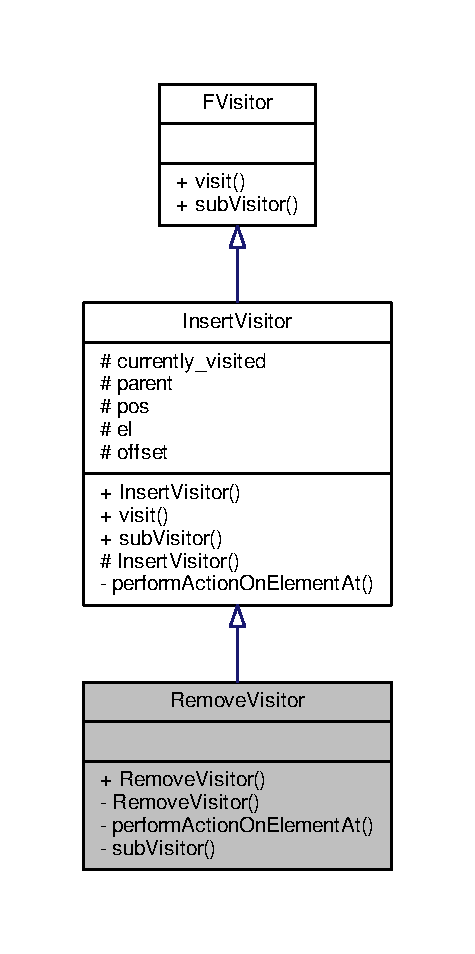
\includegraphics[width=228pt]{classRemoveVisitor__inherit__graph}
\end{center}
\end{figure}


Collaboration diagram for Remove\+Visitor\+:
\nopagebreak
\begin{figure}[H]
\begin{center}
\leavevmode
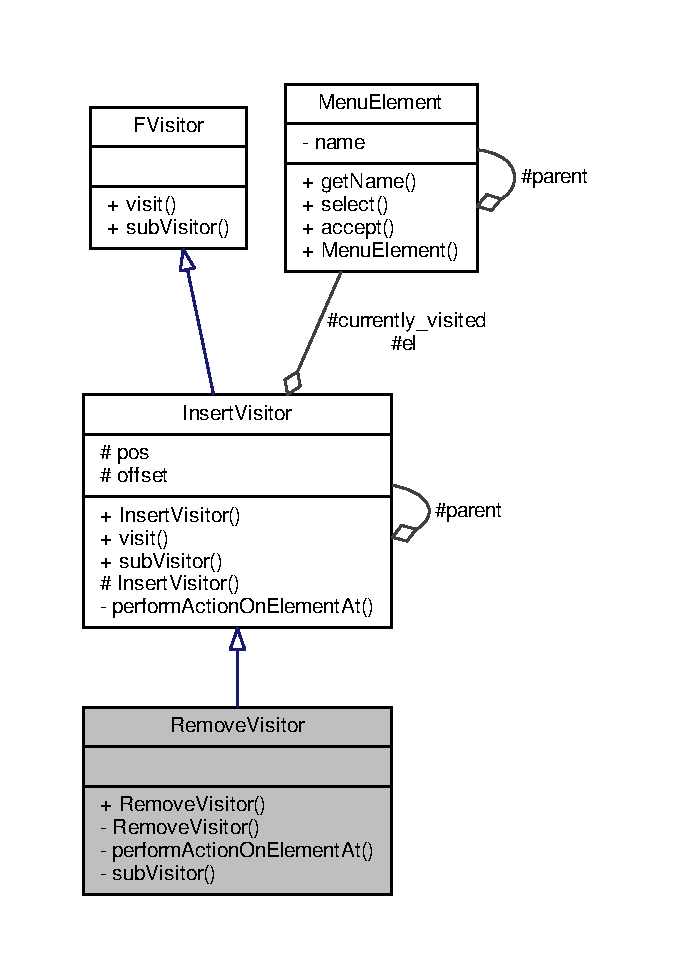
\includegraphics[width=323pt]{classRemoveVisitor__coll__graph}
\end{center}
\end{figure}
\subsection*{Public Member Functions}
\begin{DoxyCompactItemize}
\item 
\hyperlink{classRemoveVisitor_ab80c54299d03273980f7306e3c9ec7e7}{Remove\+Visitor} (uint \hyperlink{classInsertVisitor_aeb7469f88fb024421c1dd9cfd3608d7d}{pos})
\end{DoxyCompactItemize}
\subsection*{Private Member Functions}
\begin{DoxyCompactItemize}
\item 
\hyperlink{classRemoveVisitor_ad6e89a6b6b17d9aaf16b63b42d7e98f0}{Remove\+Visitor} (std\+::shared\+\_\+ptr$<$ uint $>$ \hyperlink{classInsertVisitor_aeb7469f88fb024421c1dd9cfd3608d7d}{pos}, \hyperlink{classInsertVisitor}{Insert\+Visitor} $\ast$\hyperlink{classInsertVisitor_a33db65fd081bd0448763274f1ca4632d}{parent})
\item 
virtual void \hyperlink{classRemoveVisitor_ae13ff6c08945e8e3e8d532d9cf905cfe}{perform\+Action\+On\+Element\+At} (uint \hyperlink{classInsertVisitor_a46d57991e7305aff32cc2c8033986fc2}{offset}) override
\item 
virtual std\+::unique\+\_\+ptr$<$ \hyperlink{classFVisitor}{F\+Visitor} $>$ \hyperlink{classRemoveVisitor_a44528eb89bc3150e3b322e367c1a7ffe}{sub\+Visitor} () override
\end{DoxyCompactItemize}
\subsection*{Additional Inherited Members}


\subsection{Constructor \& Destructor Documentation}
\hypertarget{classRemoveVisitor_ab80c54299d03273980f7306e3c9ec7e7}{}\index{Remove\+Visitor@{Remove\+Visitor}!Remove\+Visitor@{Remove\+Visitor}}
\index{Remove\+Visitor@{Remove\+Visitor}!Remove\+Visitor@{Remove\+Visitor}}
\subsubsection[{Remove\+Visitor}]{\setlength{\rightskip}{0pt plus 5cm}Remove\+Visitor\+::\+Remove\+Visitor (
\begin{DoxyParamCaption}
\item[{uint}]{pos}
\end{DoxyParamCaption}
)\hspace{0.3cm}{\ttfamily [inline]}}\label{classRemoveVisitor_ab80c54299d03273980f7306e3c9ec7e7}
\hypertarget{classRemoveVisitor_ad6e89a6b6b17d9aaf16b63b42d7e98f0}{}\index{Remove\+Visitor@{Remove\+Visitor}!Remove\+Visitor@{Remove\+Visitor}}
\index{Remove\+Visitor@{Remove\+Visitor}!Remove\+Visitor@{Remove\+Visitor}}
\subsubsection[{Remove\+Visitor}]{\setlength{\rightskip}{0pt plus 5cm}Remove\+Visitor\+::\+Remove\+Visitor (
\begin{DoxyParamCaption}
\item[{std\+::shared\+\_\+ptr$<$ uint $>$}]{pos, }
\item[{{\bf Insert\+Visitor} $\ast$}]{parent}
\end{DoxyParamCaption}
)\hspace{0.3cm}{\ttfamily [inline]}, {\ttfamily [private]}}\label{classRemoveVisitor_ad6e89a6b6b17d9aaf16b63b42d7e98f0}


\subsection{Member Function Documentation}
\hypertarget{classRemoveVisitor_ae13ff6c08945e8e3e8d532d9cf905cfe}{}\index{Remove\+Visitor@{Remove\+Visitor}!perform\+Action\+On\+Element\+At@{perform\+Action\+On\+Element\+At}}
\index{perform\+Action\+On\+Element\+At@{perform\+Action\+On\+Element\+At}!Remove\+Visitor@{Remove\+Visitor}}
\subsubsection[{perform\+Action\+On\+Element\+At}]{\setlength{\rightskip}{0pt plus 5cm}void Remove\+Visitor\+::perform\+Action\+On\+Element\+At (
\begin{DoxyParamCaption}
\item[{uint}]{offset}
\end{DoxyParamCaption}
)\hspace{0.3cm}{\ttfamily [override]}, {\ttfamily [private]}, {\ttfamily [virtual]}}\label{classRemoveVisitor_ae13ff6c08945e8e3e8d532d9cf905cfe}


Reimplemented from \hyperlink{classInsertVisitor_a392e3ea0fd4f20801ce0d4e1a552d378}{Insert\+Visitor}.

\hypertarget{classRemoveVisitor_a44528eb89bc3150e3b322e367c1a7ffe}{}\index{Remove\+Visitor@{Remove\+Visitor}!sub\+Visitor@{sub\+Visitor}}
\index{sub\+Visitor@{sub\+Visitor}!Remove\+Visitor@{Remove\+Visitor}}
\subsubsection[{sub\+Visitor}]{\setlength{\rightskip}{0pt plus 5cm}std\+::unique\+\_\+ptr$<$ {\bf F\+Visitor} $>$ Remove\+Visitor\+::sub\+Visitor (
\begin{DoxyParamCaption}
{}
\end{DoxyParamCaption}
)\hspace{0.3cm}{\ttfamily [override]}, {\ttfamily [private]}, {\ttfamily [virtual]}}\label{classRemoveVisitor_a44528eb89bc3150e3b322e367c1a7ffe}


Reimplemented from \hyperlink{classInsertVisitor_a6257a7684631f6ce7cf15855eb99c8f5}{Insert\+Visitor}.



The documentation for this class was generated from the following files\+:\begin{DoxyCompactItemize}
\item 
\hyperlink{RemoveVisitor_8h}{Remove\+Visitor.\+h}\item 
\hyperlink{RemoveVisitor_8cpp}{Remove\+Visitor.\+cpp}\end{DoxyCompactItemize}

\hypertarget{classSelectElementVisitor}{}\section{Select\+Element\+Visitor Class Reference}
\label{classSelectElementVisitor}\index{Select\+Element\+Visitor@{Select\+Element\+Visitor}}


{\ttfamily \#include $<$Select\+Element\+Visitor.\+h$>$}



Inheritance diagram for Select\+Element\+Visitor\+:
\nopagebreak
\begin{figure}[H]
\begin{center}
\leavevmode
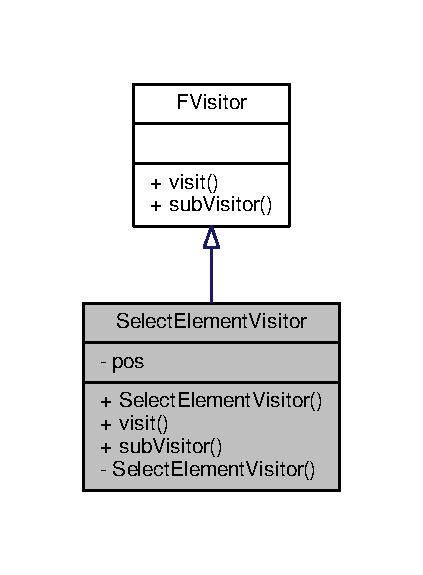
\includegraphics[width=203pt]{classSelectElementVisitor__inherit__graph}
\end{center}
\end{figure}


Collaboration diagram for Select\+Element\+Visitor\+:
\nopagebreak
\begin{figure}[H]
\begin{center}
\leavevmode
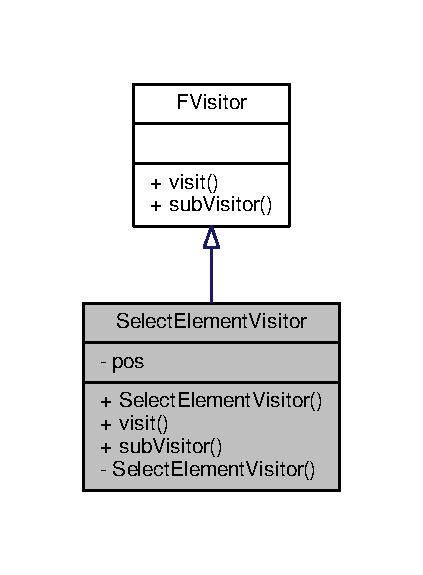
\includegraphics[width=203pt]{classSelectElementVisitor__coll__graph}
\end{center}
\end{figure}
\subsection*{Public Member Functions}
\begin{DoxyCompactItemize}
\item 
\hyperlink{classSelectElementVisitor_a4f37877d76bd362bdc5168eda70a4f6f}{Select\+Element\+Visitor} (uint \hyperlink{classSelectElementVisitor_a6a3a2d25639fe5e0112a52b3622d2cb1}{pos})
\item 
virtual void \hyperlink{classSelectElementVisitor_af2dabf443aa6b32b253ca05baf3b780f}{visit} (\hyperlink{classMenuElement}{Menu\+Element} $\ast$element)
\item 
virtual std\+::unique\+\_\+ptr$<$ \hyperlink{classFVisitor}{F\+Visitor} $>$ \hyperlink{classSelectElementVisitor_afa97120c24b6f67f81dfdb65bd243949}{sub\+Visitor} ()
\end{DoxyCompactItemize}
\subsection*{Private Member Functions}
\begin{DoxyCompactItemize}
\item 
\hyperlink{classSelectElementVisitor_aab7a8b4f9292063876c4884964d21592}{Select\+Element\+Visitor} (std\+::shared\+\_\+ptr$<$ uint $>$ \hyperlink{classSelectElementVisitor_a6a3a2d25639fe5e0112a52b3622d2cb1}{pos})
\end{DoxyCompactItemize}
\subsection*{Private Attributes}
\begin{DoxyCompactItemize}
\item 
std\+::shared\+\_\+ptr$<$ uint $>$ \hyperlink{classSelectElementVisitor_a6a3a2d25639fe5e0112a52b3622d2cb1}{pos}
\end{DoxyCompactItemize}


\subsection{Constructor \& Destructor Documentation}
\hypertarget{classSelectElementVisitor_a4f37877d76bd362bdc5168eda70a4f6f}{}\index{Select\+Element\+Visitor@{Select\+Element\+Visitor}!Select\+Element\+Visitor@{Select\+Element\+Visitor}}
\index{Select\+Element\+Visitor@{Select\+Element\+Visitor}!Select\+Element\+Visitor@{Select\+Element\+Visitor}}
\subsubsection[{Select\+Element\+Visitor}]{\setlength{\rightskip}{0pt plus 5cm}Select\+Element\+Visitor\+::\+Select\+Element\+Visitor (
\begin{DoxyParamCaption}
\item[{uint}]{pos}
\end{DoxyParamCaption}
)\hspace{0.3cm}{\ttfamily [inline]}}\label{classSelectElementVisitor_a4f37877d76bd362bdc5168eda70a4f6f}
\hypertarget{classSelectElementVisitor_aab7a8b4f9292063876c4884964d21592}{}\index{Select\+Element\+Visitor@{Select\+Element\+Visitor}!Select\+Element\+Visitor@{Select\+Element\+Visitor}}
\index{Select\+Element\+Visitor@{Select\+Element\+Visitor}!Select\+Element\+Visitor@{Select\+Element\+Visitor}}
\subsubsection[{Select\+Element\+Visitor}]{\setlength{\rightskip}{0pt plus 5cm}Select\+Element\+Visitor\+::\+Select\+Element\+Visitor (
\begin{DoxyParamCaption}
\item[{std\+::shared\+\_\+ptr$<$ uint $>$}]{pos}
\end{DoxyParamCaption}
)\hspace{0.3cm}{\ttfamily [inline]}, {\ttfamily [private]}}\label{classSelectElementVisitor_aab7a8b4f9292063876c4884964d21592}


\subsection{Member Function Documentation}
\hypertarget{classSelectElementVisitor_afa97120c24b6f67f81dfdb65bd243949}{}\index{Select\+Element\+Visitor@{Select\+Element\+Visitor}!sub\+Visitor@{sub\+Visitor}}
\index{sub\+Visitor@{sub\+Visitor}!Select\+Element\+Visitor@{Select\+Element\+Visitor}}
\subsubsection[{sub\+Visitor}]{\setlength{\rightskip}{0pt plus 5cm}std\+::unique\+\_\+ptr$<$ {\bf F\+Visitor} $>$ Select\+Element\+Visitor\+::sub\+Visitor (
\begin{DoxyParamCaption}
{}
\end{DoxyParamCaption}
)\hspace{0.3cm}{\ttfamily [virtual]}}\label{classSelectElementVisitor_afa97120c24b6f67f81dfdb65bd243949}


Implements \hyperlink{classFVisitor_ae7b318528ba0bd915a0c4958eb3fe437}{F\+Visitor}.

\hypertarget{classSelectElementVisitor_af2dabf443aa6b32b253ca05baf3b780f}{}\index{Select\+Element\+Visitor@{Select\+Element\+Visitor}!visit@{visit}}
\index{visit@{visit}!Select\+Element\+Visitor@{Select\+Element\+Visitor}}
\subsubsection[{visit}]{\setlength{\rightskip}{0pt plus 5cm}void Select\+Element\+Visitor\+::visit (
\begin{DoxyParamCaption}
\item[{{\bf Menu\+Element} $\ast$}]{element}
\end{DoxyParamCaption}
)\hspace{0.3cm}{\ttfamily [virtual]}}\label{classSelectElementVisitor_af2dabf443aa6b32b253ca05baf3b780f}


Implements \hyperlink{classFVisitor_a42b99a5f7354fcd014eb44951d778058}{F\+Visitor}.



\subsection{Member Data Documentation}
\hypertarget{classSelectElementVisitor_a6a3a2d25639fe5e0112a52b3622d2cb1}{}\index{Select\+Element\+Visitor@{Select\+Element\+Visitor}!pos@{pos}}
\index{pos@{pos}!Select\+Element\+Visitor@{Select\+Element\+Visitor}}
\subsubsection[{pos}]{\setlength{\rightskip}{0pt plus 5cm}std\+::shared\+\_\+ptr$<$uint$>$ Select\+Element\+Visitor\+::pos\hspace{0.3cm}{\ttfamily [private]}}\label{classSelectElementVisitor_a6a3a2d25639fe5e0112a52b3622d2cb1}


The documentation for this class was generated from the following files\+:\begin{DoxyCompactItemize}
\item 
\hyperlink{SelectElementVisitor_8h}{Select\+Element\+Visitor.\+h}\item 
\hyperlink{SelectElementVisitor_8cpp}{Select\+Element\+Visitor.\+cpp}\end{DoxyCompactItemize}

\chapter{File Documentation}
\hypertarget{FMenuFacade_8cpp}{}\section{F\+Menu\+Facade.\+cpp File Reference}
\label{FMenuFacade_8cpp}\index{F\+Menu\+Facade.\+cpp@{F\+Menu\+Facade.\+cpp}}
{\ttfamily \#include $<$sstream$>$}\\*
{\ttfamily \#include \char`\"{}F\+Menu\+Facade.\+h\char`\"{}}\\*
{\ttfamily \#include \char`\"{}Menu\+Multi\+Select.\+h\char`\"{}}\\*
{\ttfamily \#include \char`\"{}Menu\+Single\+Select.\+h\char`\"{}}\\*
{\ttfamily \#include \char`\"{}Menu\+Name\+Visitor.\+h\char`\"{}}\\*
{\ttfamily \#include \char`\"{}Insert\+Visitor.\+h\char`\"{}}\\*
{\ttfamily \#include \char`\"{}Remove\+Visitor.\+h\char`\"{}}\\*
{\ttfamily \#include \char`\"{}Select\+Element\+Visitor.\+h\char`\"{}}\\*
Include dependency graph for F\+Menu\+Facade.\+cpp\+:
\nopagebreak
\begin{figure}[H]
\begin{center}
\leavevmode
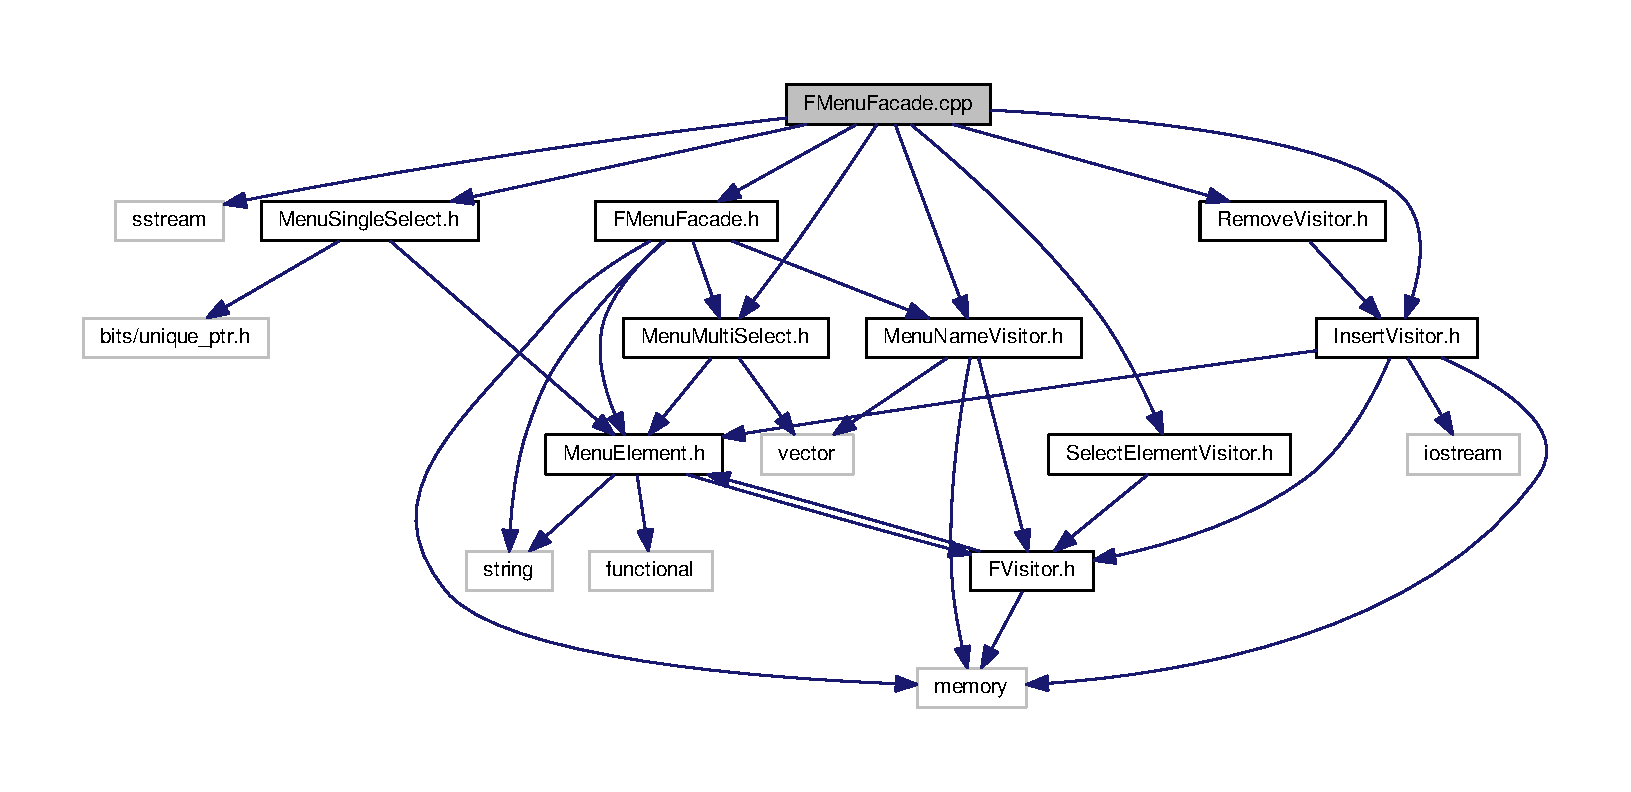
\includegraphics[width=350pt]{FMenuFacade_8cpp__incl}
\end{center}
\end{figure}
\subsection*{Functions}
\begin{DoxyCompactItemize}
\item 
std\+::ostream \& \hyperlink{FMenuFacade_8cpp_a458848f52cf6b3a97527f2bf59478542}{operator$<$$<$} (std\+::ostream \&os, const \hyperlink{classFMenuFacade_ad7061aee91a27742df50a0ee7c0201d2}{F\+Menu\+Facade\+::name} \&name)
\end{DoxyCompactItemize}


\subsection{Function Documentation}
\hypertarget{FMenuFacade_8cpp_a458848f52cf6b3a97527f2bf59478542}{}\index{F\+Menu\+Facade.\+cpp@{F\+Menu\+Facade.\+cpp}!operator$<$$<$@{operator$<$$<$}}
\index{operator$<$$<$@{operator$<$$<$}!F\+Menu\+Facade.\+cpp@{F\+Menu\+Facade.\+cpp}}
\subsubsection[{operator$<$$<$}]{\setlength{\rightskip}{0pt plus 5cm}std\+::ostream\& operator$<$$<$ (
\begin{DoxyParamCaption}
\item[{std\+::ostream \&}]{os, }
\item[{const {\bf F\+Menu\+Facade\+::name} \&}]{name}
\end{DoxyParamCaption}
)}\label{FMenuFacade_8cpp_a458848f52cf6b3a97527f2bf59478542}

\hypertarget{FMenuFacade_8h}{}\section{F\+Menu\+Facade.\+h File Reference}
\label{FMenuFacade_8h}\index{F\+Menu\+Facade.\+h@{F\+Menu\+Facade.\+h}}
{\ttfamily \#include \char`\"{}Menu\+Element.\+h\char`\"{}}\\*
{\ttfamily \#include \char`\"{}Menu\+Multi\+Select.\+h\char`\"{}}\\*
{\ttfamily \#include \char`\"{}Menu\+Name\+Visitor.\+h\char`\"{}}\\*
{\ttfamily \#include $<$memory$>$}\\*
{\ttfamily \#include $<$string$>$}\\*
Include dependency graph for F\+Menu\+Facade.\+h\+:
\nopagebreak
\begin{figure}[H]
\begin{center}
\leavevmode
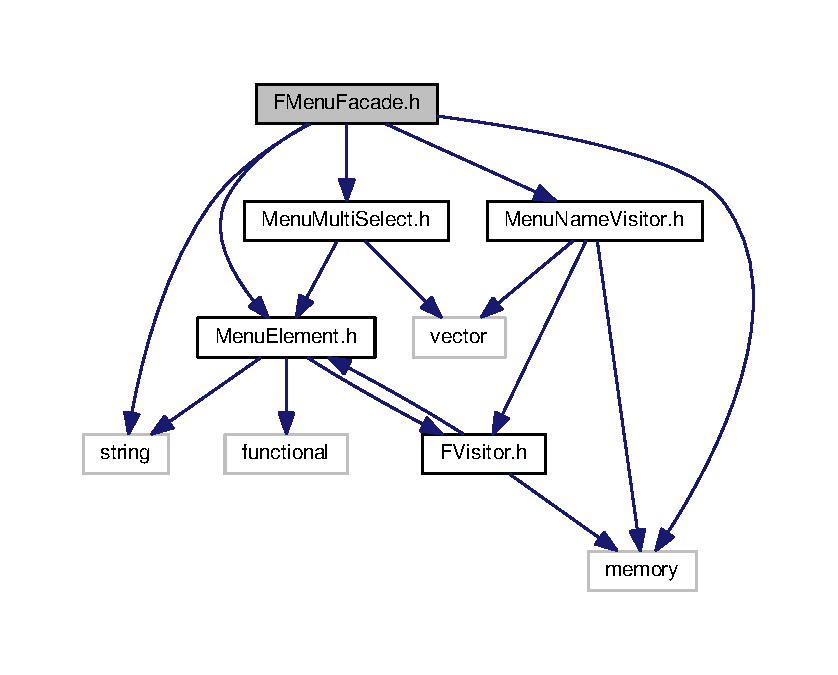
\includegraphics[width=350pt]{FMenuFacade_8h__incl}
\end{center}
\end{figure}
This graph shows which files directly or indirectly include this file\+:
\nopagebreak
\begin{figure}[H]
\begin{center}
\leavevmode
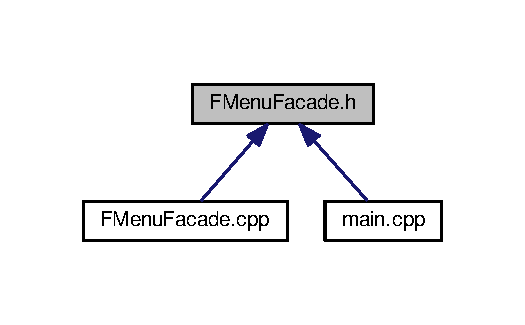
\includegraphics[width=252pt]{FMenuFacade_8h__dep__incl}
\end{center}
\end{figure}
\subsection*{Classes}
\begin{DoxyCompactItemize}
\item 
class \hyperlink{classFMenuFacade}{F\+Menu\+Facade}
\end{DoxyCompactItemize}
\subsection*{Functions}
\begin{DoxyCompactItemize}
\item 
std\+::ostream \& \hyperlink{FMenuFacade_8h_aa88e569dc8dc251d2bf69db257d70fc5}{operator$<$$<$} (std\+::ostream \&out, const \hyperlink{classFMenuFacade_ad7061aee91a27742df50a0ee7c0201d2}{F\+Menu\+Facade\+::name} \&)
\end{DoxyCompactItemize}


\subsection{Function Documentation}
\hypertarget{FMenuFacade_8h_aa88e569dc8dc251d2bf69db257d70fc5}{}\index{F\+Menu\+Facade.\+h@{F\+Menu\+Facade.\+h}!operator$<$$<$@{operator$<$$<$}}
\index{operator$<$$<$@{operator$<$$<$}!F\+Menu\+Facade.\+h@{F\+Menu\+Facade.\+h}}
\subsubsection[{operator$<$$<$}]{\setlength{\rightskip}{0pt plus 5cm}std\+::ostream\& operator$<$$<$ (
\begin{DoxyParamCaption}
\item[{std\+::ostream \&}]{out, }
\item[{const {\bf F\+Menu\+Facade\+::name} \&}]{}
\end{DoxyParamCaption}
)}\label{FMenuFacade_8h_aa88e569dc8dc251d2bf69db257d70fc5}

\hypertarget{FVisitor_8cpp}{}\section{F\+Visitor.\+cpp File Reference}
\label{FVisitor_8cpp}\index{F\+Visitor.\+cpp@{F\+Visitor.\+cpp}}
{\ttfamily \#include \char`\"{}F\+Visitor.\+h\char`\"{}}\\*
Include dependency graph for F\+Visitor.\+cpp\+:
\nopagebreak
\begin{figure}[H]
\begin{center}
\leavevmode
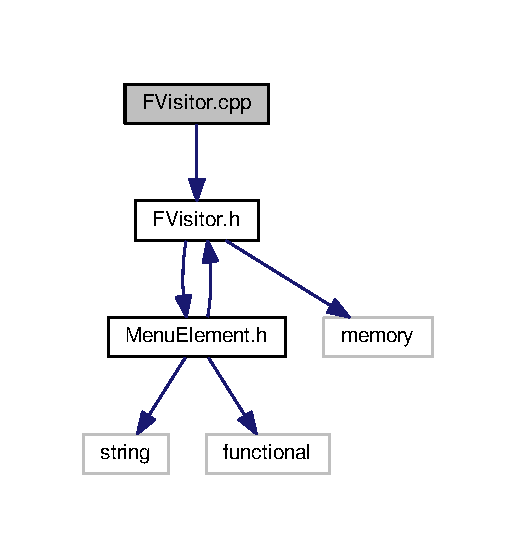
\includegraphics[width=248pt]{FVisitor_8cpp__incl}
\end{center}
\end{figure}

\hypertarget{FVisitor_8h}{}\section{F\+Visitor.\+h File Reference}
\label{FVisitor_8h}\index{F\+Visitor.\+h@{F\+Visitor.\+h}}
{\ttfamily \#include \char`\"{}Menu\+Element.\+h\char`\"{}}\\*
{\ttfamily \#include $<$memory$>$}\\*
Include dependency graph for F\+Visitor.\+h\+:
\nopagebreak
\begin{figure}[H]
\begin{center}
\leavevmode
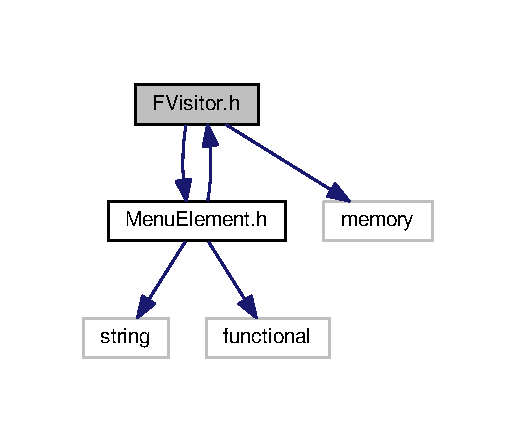
\includegraphics[width=248pt]{FVisitor_8h__incl}
\end{center}
\end{figure}
This graph shows which files directly or indirectly include this file\+:
\nopagebreak
\begin{figure}[H]
\begin{center}
\leavevmode
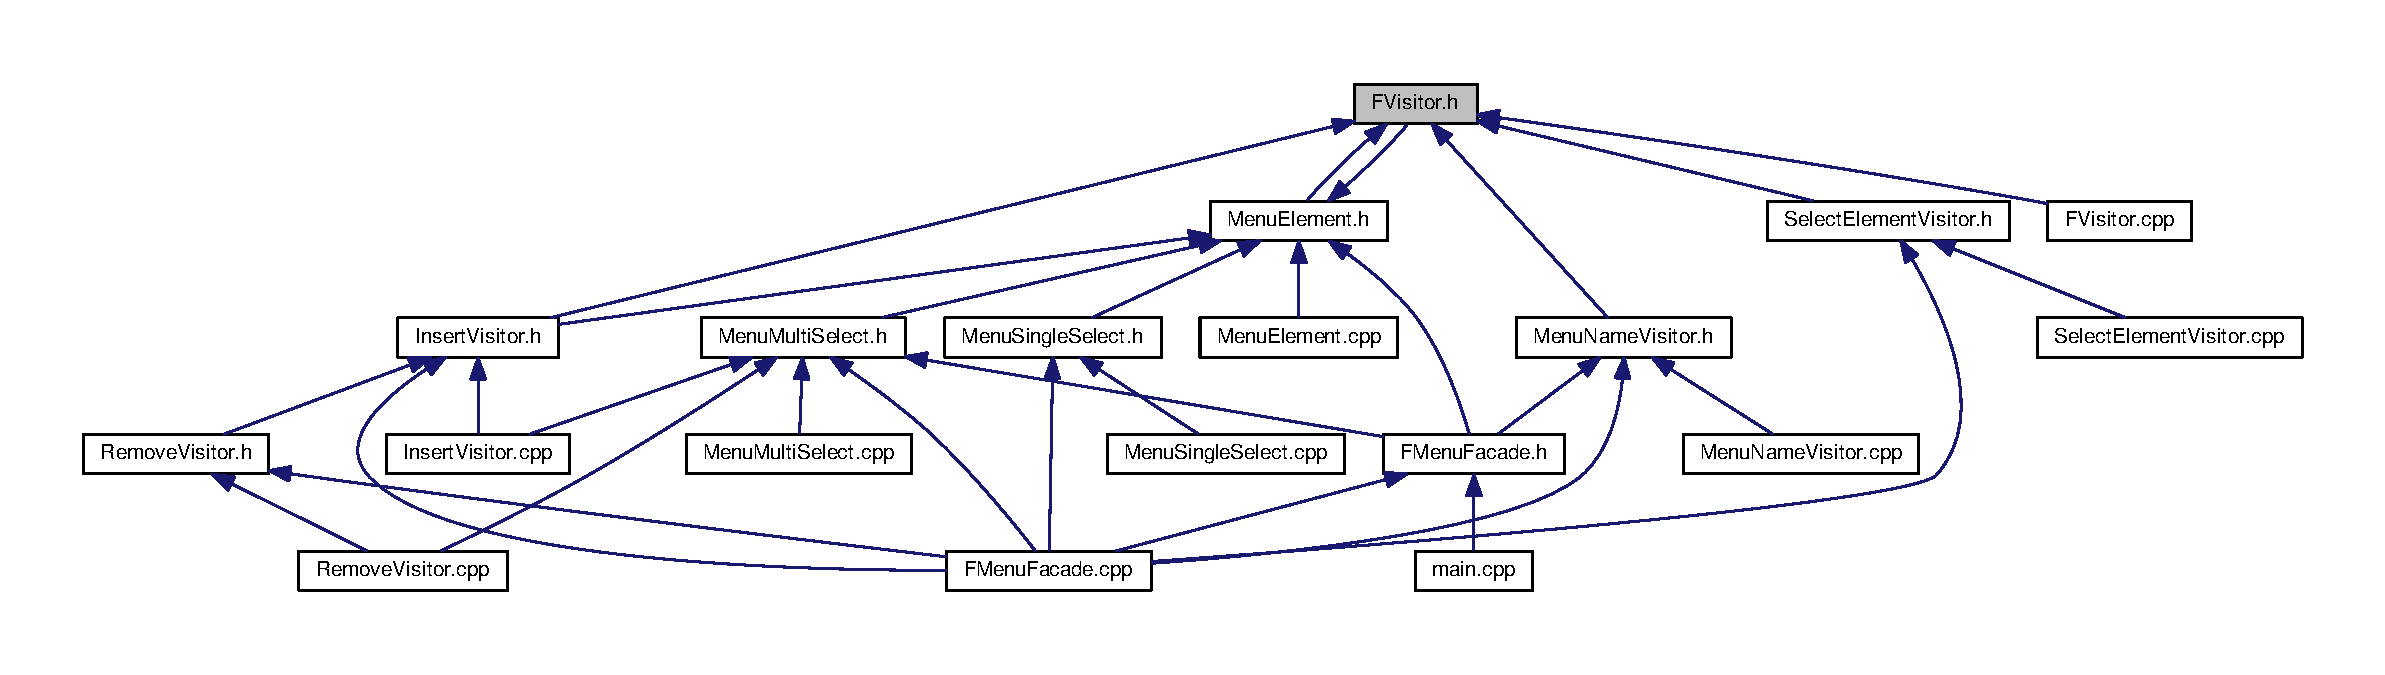
\includegraphics[width=350pt]{FVisitor_8h__dep__incl}
\end{center}
\end{figure}
\subsection*{Classes}
\begin{DoxyCompactItemize}
\item 
class \hyperlink{classFVisitor}{F\+Visitor}
\end{DoxyCompactItemize}

\hypertarget{InsertVisitor_8cpp}{}\section{Insert\+Visitor.\+cpp File Reference}
\label{InsertVisitor_8cpp}\index{Insert\+Visitor.\+cpp@{Insert\+Visitor.\+cpp}}
{\ttfamily \#include \char`\"{}Insert\+Visitor.\+h\char`\"{}}\\*
{\ttfamily \#include \char`\"{}Menu\+Multi\+Select.\+h\char`\"{}}\\*
{\ttfamily \#include $<$iostream$>$}\\*
Include dependency graph for Insert\+Visitor.\+cpp\+:
\nopagebreak
\begin{figure}[H]
\begin{center}
\leavevmode
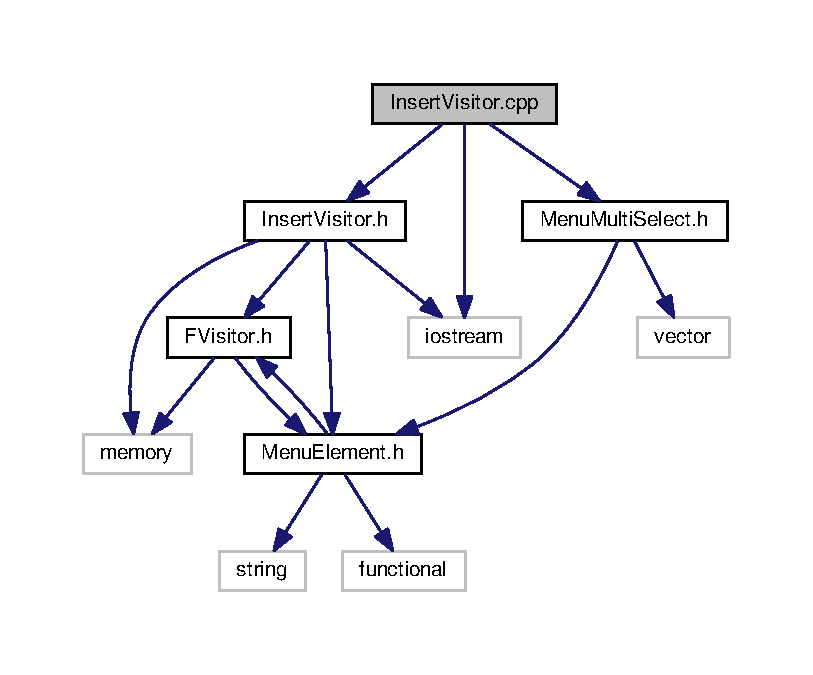
\includegraphics[width=350pt]{InsertVisitor_8cpp__incl}
\end{center}
\end{figure}

\hypertarget{InsertVisitor_8h}{}\section{Insert\+Visitor.\+h File Reference}
\label{InsertVisitor_8h}\index{Insert\+Visitor.\+h@{Insert\+Visitor.\+h}}
{\ttfamily \#include \char`\"{}F\+Visitor.\+h\char`\"{}}\\*
{\ttfamily \#include \char`\"{}Menu\+Element.\+h\char`\"{}}\\*
{\ttfamily \#include $<$memory$>$}\\*
{\ttfamily \#include $<$iostream$>$}\\*
Include dependency graph for Insert\+Visitor.\+h\+:
\nopagebreak
\begin{figure}[H]
\begin{center}
\leavevmode
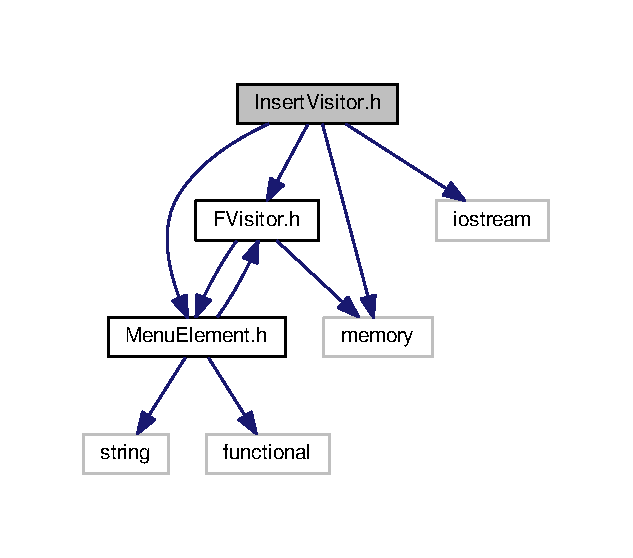
\includegraphics[width=304pt]{InsertVisitor_8h__incl}
\end{center}
\end{figure}
This graph shows which files directly or indirectly include this file\+:
\nopagebreak
\begin{figure}[H]
\begin{center}
\leavevmode
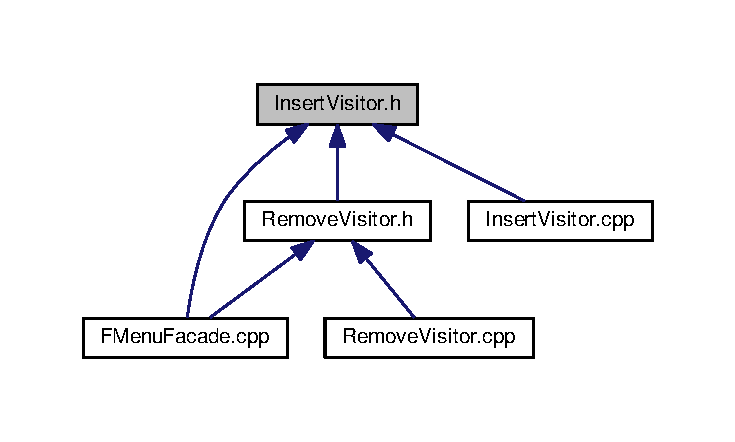
\includegraphics[width=350pt]{InsertVisitor_8h__dep__incl}
\end{center}
\end{figure}
\subsection*{Classes}
\begin{DoxyCompactItemize}
\item 
class \hyperlink{classInsertVisitor}{Insert\+Visitor}
\end{DoxyCompactItemize}

\hypertarget{main_8cpp}{}\section{main.\+cpp File Reference}
\label{main_8cpp}\index{main.\+cpp@{main.\+cpp}}
{\ttfamily \#include $<$iostream$>$}\\*
{\ttfamily \#include \char`\"{}F\+Menu\+Facade.\+h\char`\"{}}\\*
Include dependency graph for main.\+cpp\+:
\nopagebreak
\begin{figure}[H]
\begin{center}
\leavevmode
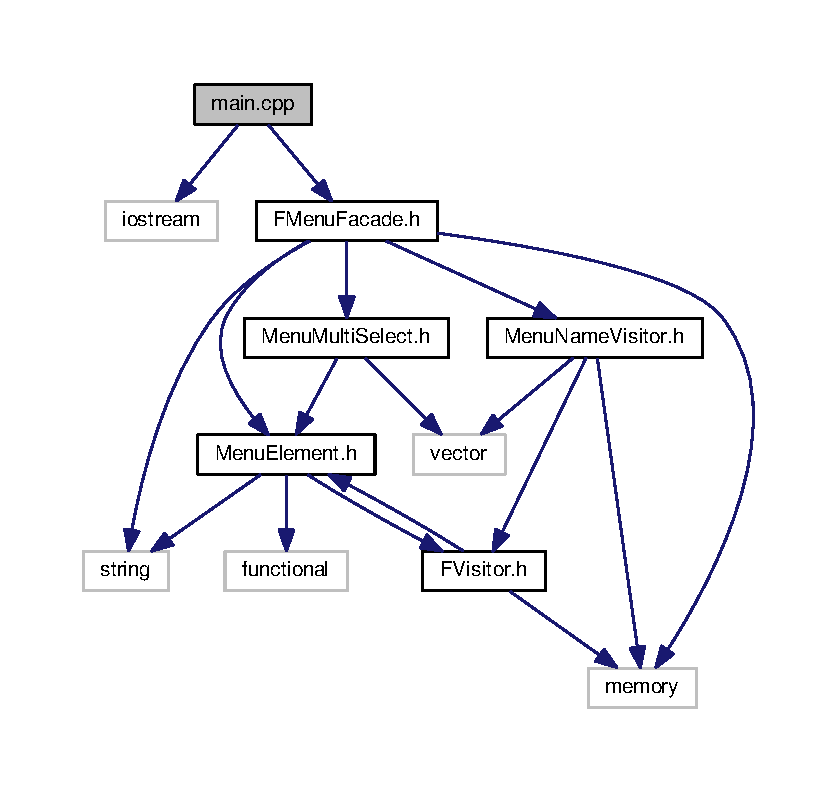
\includegraphics[width=350pt]{main_8cpp__incl}
\end{center}
\end{figure}
\subsection*{Functions}
\begin{DoxyCompactItemize}
\item 
int \hyperlink{main_8cpp_ae66f6b31b5ad750f1fe042a706a4e3d4}{main} ()
\end{DoxyCompactItemize}


\subsection{Function Documentation}
\hypertarget{main_8cpp_ae66f6b31b5ad750f1fe042a706a4e3d4}{}\index{main.\+cpp@{main.\+cpp}!main@{main}}
\index{main@{main}!main.\+cpp@{main.\+cpp}}
\subsubsection[{main}]{\setlength{\rightskip}{0pt plus 5cm}int main (
\begin{DoxyParamCaption}
{}
\end{DoxyParamCaption}
)}\label{main_8cpp_ae66f6b31b5ad750f1fe042a706a4e3d4}

\hypertarget{MenuElement_8cpp}{}\section{Menu\+Element.\+cpp File Reference}
\label{MenuElement_8cpp}\index{Menu\+Element.\+cpp@{Menu\+Element.\+cpp}}
{\ttfamily \#include \char`\"{}Menu\+Element.\+h\char`\"{}}\\*
Include dependency graph for Menu\+Element.\+cpp\+:
\nopagebreak
\begin{figure}[H]
\begin{center}
\leavevmode
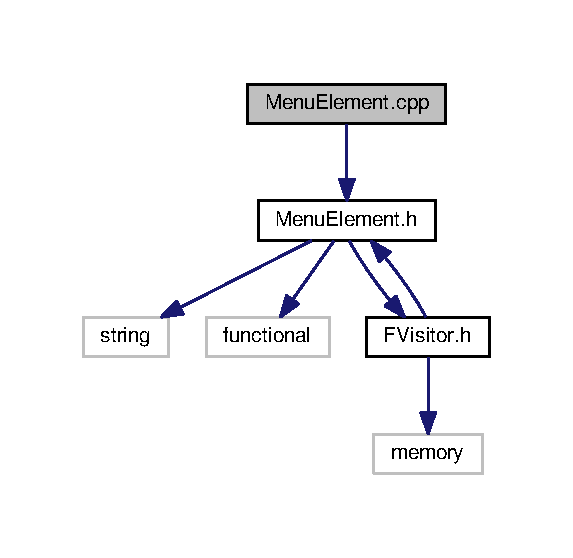
\includegraphics[width=275pt]{MenuElement_8cpp__incl}
\end{center}
\end{figure}

\hypertarget{MenuElement_8h}{}\section{Menu\+Element.\+h File Reference}
\label{MenuElement_8h}\index{Menu\+Element.\+h@{Menu\+Element.\+h}}
{\ttfamily \#include $<$string$>$}\\*
{\ttfamily \#include $<$functional$>$}\\*
{\ttfamily \#include \char`\"{}F\+Visitor.\+h\char`\"{}}\\*
Include dependency graph for Menu\+Element.\+h\+:
\nopagebreak
\begin{figure}[H]
\begin{center}
\leavevmode
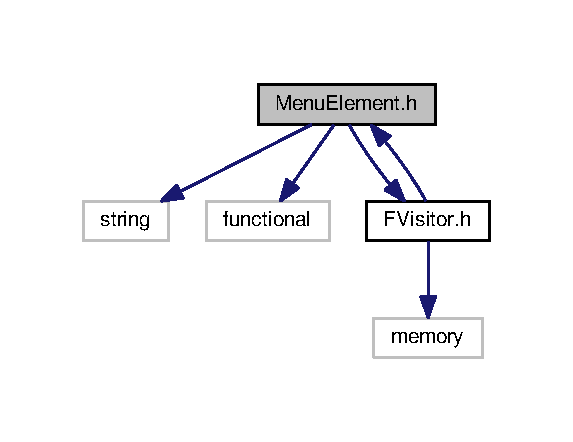
\includegraphics[width=275pt]{MenuElement_8h__incl}
\end{center}
\end{figure}
This graph shows which files directly or indirectly include this file\+:
\nopagebreak
\begin{figure}[H]
\begin{center}
\leavevmode
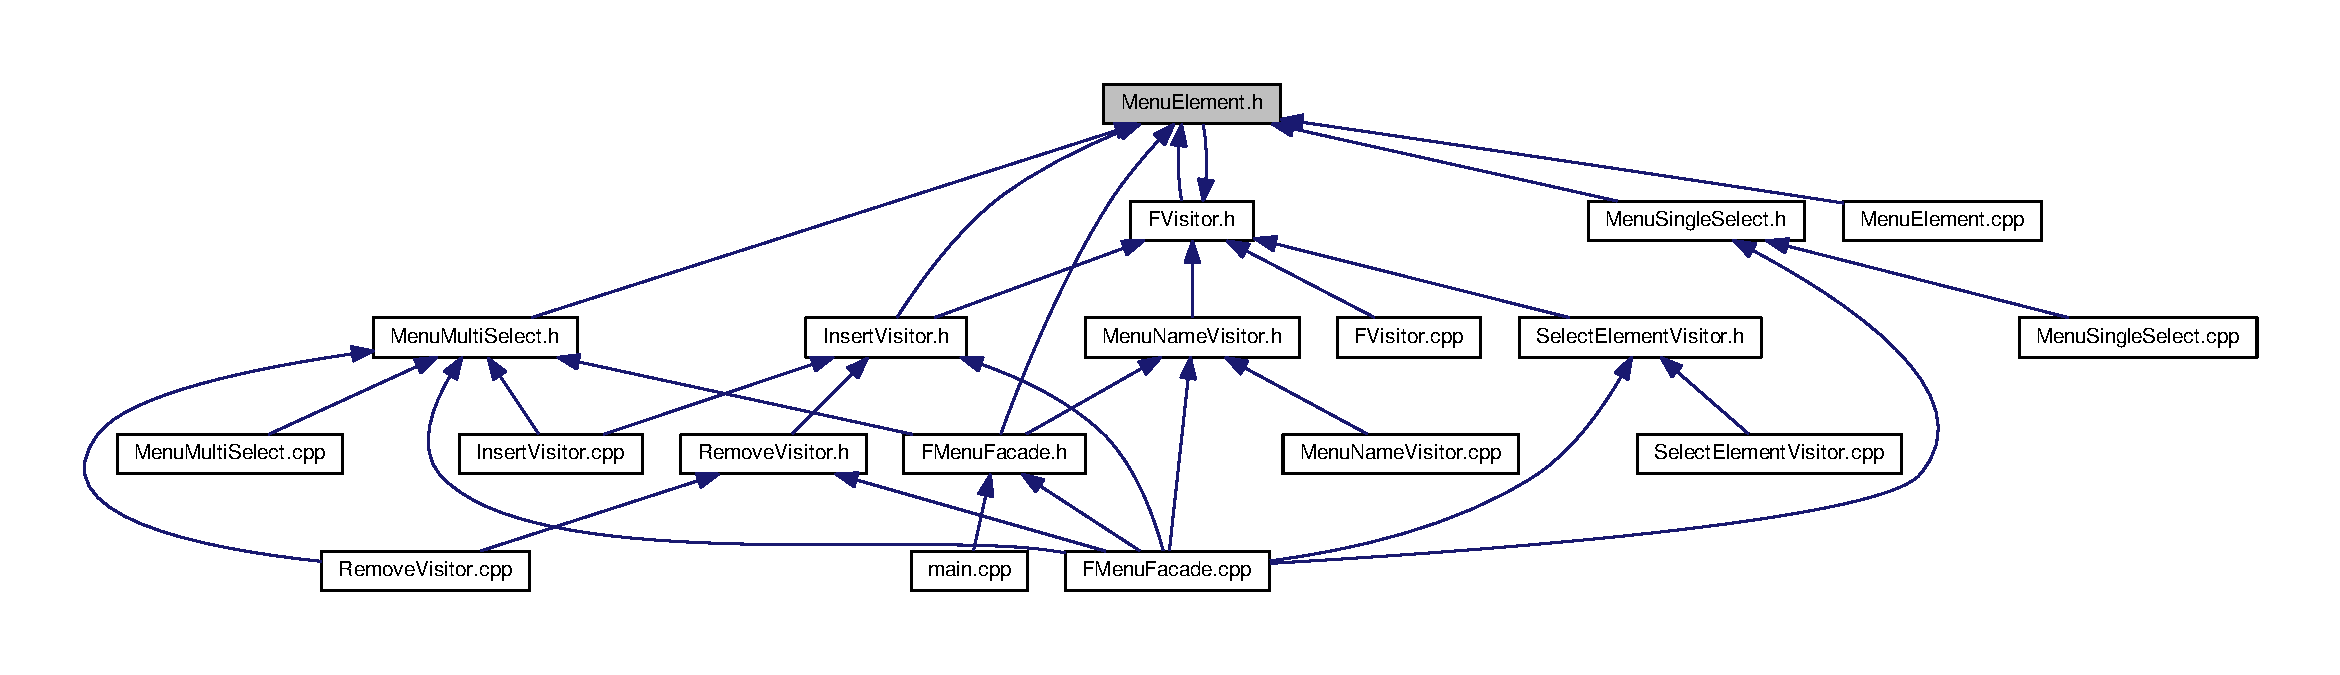
\includegraphics[width=350pt]{MenuElement_8h__dep__incl}
\end{center}
\end{figure}
\subsection*{Classes}
\begin{DoxyCompactItemize}
\item 
class \hyperlink{classMenuElement}{Menu\+Element}
\end{DoxyCompactItemize}

\hypertarget{MenuMultiSelect_8cpp}{}\section{Menu\+Multi\+Select.\+cpp File Reference}
\label{MenuMultiSelect_8cpp}\index{Menu\+Multi\+Select.\+cpp@{Menu\+Multi\+Select.\+cpp}}
{\ttfamily \#include \char`\"{}Menu\+Multi\+Select.\+h\char`\"{}}\\*
{\ttfamily \#include $<$algorithm$>$}\\*
{\ttfamily \#include $<$iostream$>$}\\*
{\ttfamily \#include $<$assert.\+h$>$}\\*
Include dependency graph for Menu\+Multi\+Select.\+cpp\+:
\nopagebreak
\begin{figure}[H]
\begin{center}
\leavevmode
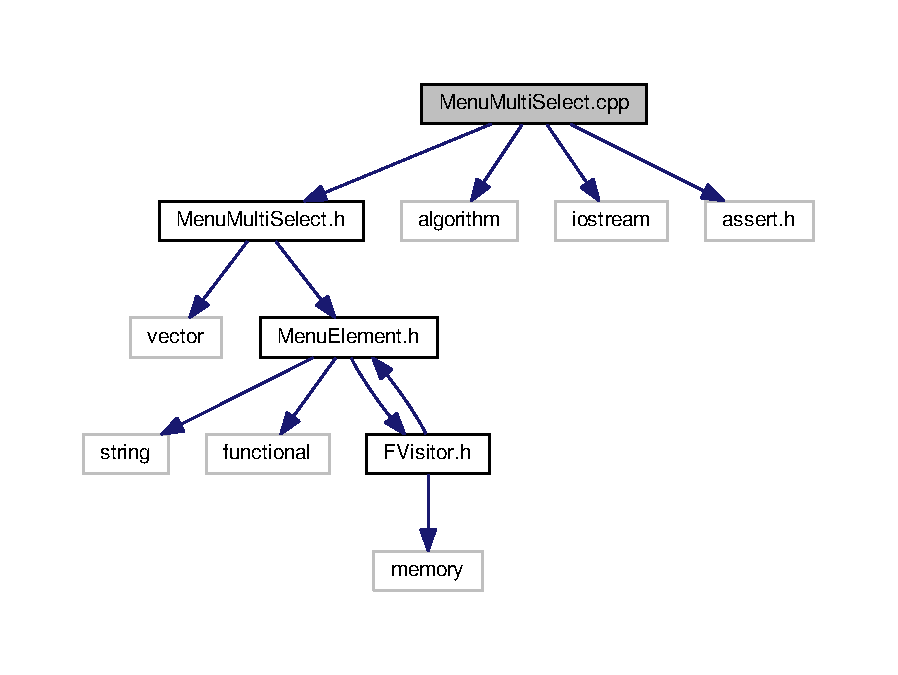
\includegraphics[width=350pt]{MenuMultiSelect_8cpp__incl}
\end{center}
\end{figure}

\hypertarget{MenuMultiSelect_8h}{}\section{Menu\+Multi\+Select.\+h File Reference}
\label{MenuMultiSelect_8h}\index{Menu\+Multi\+Select.\+h@{Menu\+Multi\+Select.\+h}}
{\ttfamily \#include $<$vector$>$}\\*
{\ttfamily \#include \char`\"{}Menu\+Element.\+h\char`\"{}}\\*
Include dependency graph for Menu\+Multi\+Select.\+h\+:
\nopagebreak
\begin{figure}[H]
\begin{center}
\leavevmode
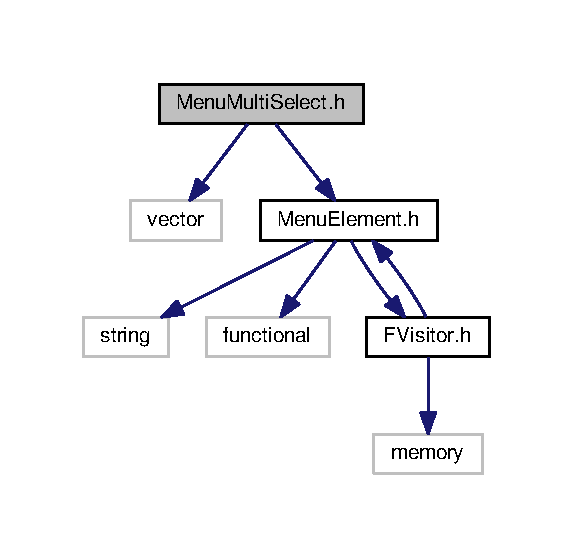
\includegraphics[width=275pt]{MenuMultiSelect_8h__incl}
\end{center}
\end{figure}
This graph shows which files directly or indirectly include this file\+:
\nopagebreak
\begin{figure}[H]
\begin{center}
\leavevmode
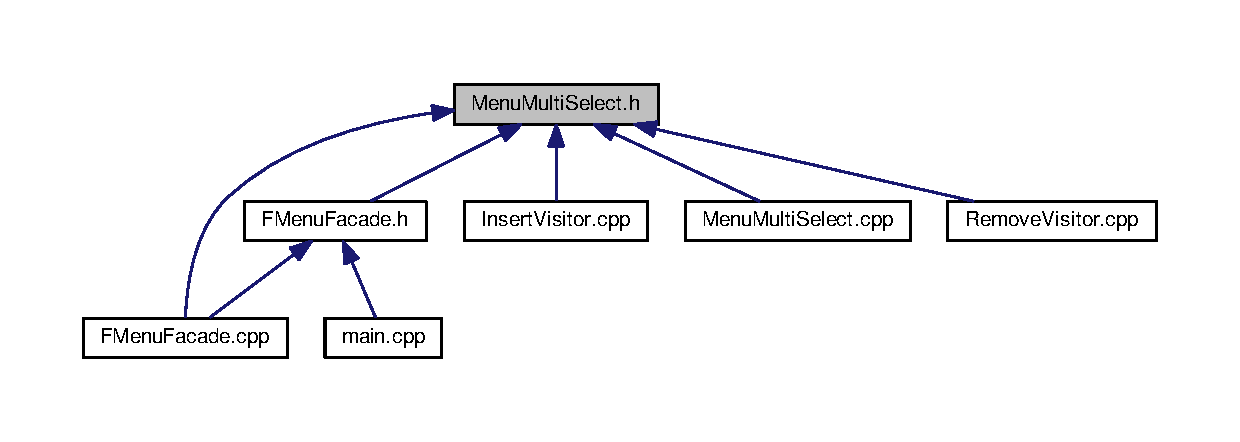
\includegraphics[width=350pt]{MenuMultiSelect_8h__dep__incl}
\end{center}
\end{figure}
\subsection*{Classes}
\begin{DoxyCompactItemize}
\item 
class \hyperlink{classMenuMultiSelect}{Menu\+Multi\+Select}
\end{DoxyCompactItemize}

\hypertarget{MenuNameVisitor_8cpp}{}\section{Menu\+Name\+Visitor.\+cpp File Reference}
\label{MenuNameVisitor_8cpp}\index{Menu\+Name\+Visitor.\+cpp@{Menu\+Name\+Visitor.\+cpp}}
{\ttfamily \#include $<$sstream$>$}\\*
{\ttfamily \#include \char`\"{}Menu\+Name\+Visitor.\+h\char`\"{}}\\*
Include dependency graph for Menu\+Name\+Visitor.\+cpp\+:
\nopagebreak
\begin{figure}[H]
\begin{center}
\leavevmode
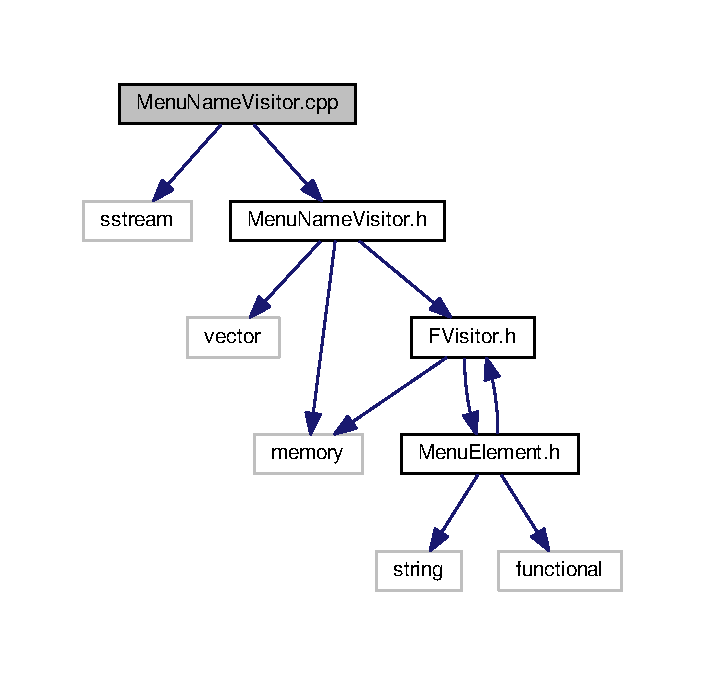
\includegraphics[width=339pt]{MenuNameVisitor_8cpp__incl}
\end{center}
\end{figure}

\hypertarget{MenuNameVisitor_8h}{}\section{Menu\+Name\+Visitor.\+h File Reference}
\label{MenuNameVisitor_8h}\index{Menu\+Name\+Visitor.\+h@{Menu\+Name\+Visitor.\+h}}
{\ttfamily \#include $<$vector$>$}\\*
{\ttfamily \#include $<$memory$>$}\\*
{\ttfamily \#include \char`\"{}F\+Visitor.\+h\char`\"{}}\\*
Include dependency graph for Menu\+Name\+Visitor.\+h\+:
\nopagebreak
\begin{figure}[H]
\begin{center}
\leavevmode
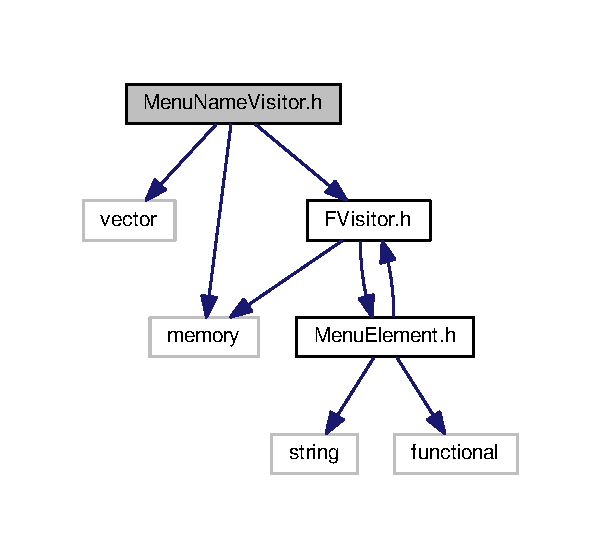
\includegraphics[width=289pt]{MenuNameVisitor_8h__incl}
\end{center}
\end{figure}
This graph shows which files directly or indirectly include this file\+:
\nopagebreak
\begin{figure}[H]
\begin{center}
\leavevmode
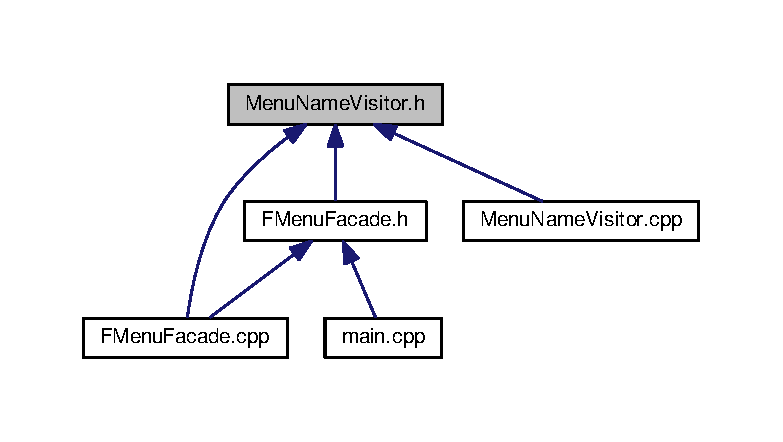
\includegraphics[width=350pt]{MenuNameVisitor_8h__dep__incl}
\end{center}
\end{figure}
\subsection*{Classes}
\begin{DoxyCompactItemize}
\item 
class \hyperlink{classMenuNameVisitor}{Menu\+Name\+Visitor}
\end{DoxyCompactItemize}

\hypertarget{MenuSingleSelect_8cpp}{}\section{Menu\+Single\+Select.\+cpp File Reference}
\label{MenuSingleSelect_8cpp}\index{Menu\+Single\+Select.\+cpp@{Menu\+Single\+Select.\+cpp}}
{\ttfamily \#include \char`\"{}Menu\+Single\+Select.\+h\char`\"{}}\\*
Include dependency graph for Menu\+Single\+Select.\+cpp\+:
\nopagebreak
\begin{figure}[H]
\begin{center}
\leavevmode
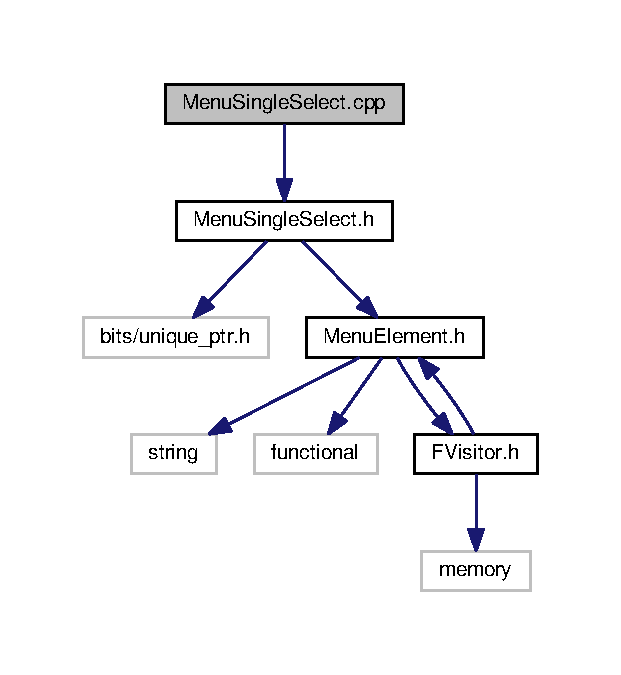
\includegraphics[width=298pt]{MenuSingleSelect_8cpp__incl}
\end{center}
\end{figure}

\hypertarget{MenuSingleSelect_8h}{}\section{Menu\+Single\+Select.\+h File Reference}
\label{MenuSingleSelect_8h}\index{Menu\+Single\+Select.\+h@{Menu\+Single\+Select.\+h}}
{\ttfamily \#include $<$bits/unique\+\_\+ptr.\+h$>$}\\*
{\ttfamily \#include \char`\"{}Menu\+Element.\+h\char`\"{}}\\*
Include dependency graph for Menu\+Single\+Select.\+h\+:
\nopagebreak
\begin{figure}[H]
\begin{center}
\leavevmode
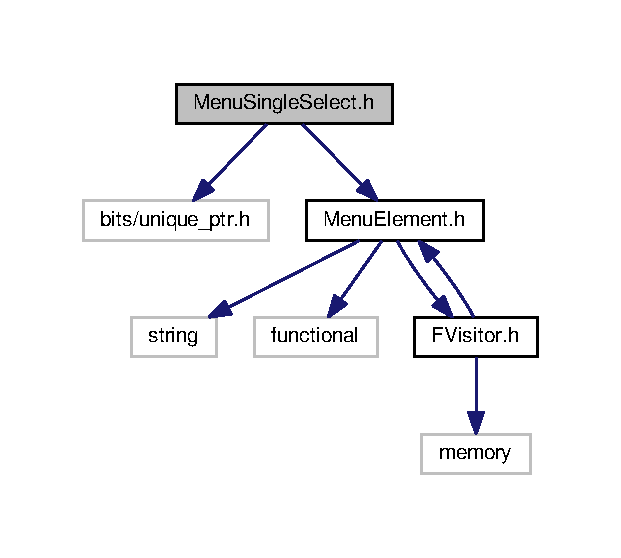
\includegraphics[width=298pt]{MenuSingleSelect_8h__incl}
\end{center}
\end{figure}
This graph shows which files directly or indirectly include this file\+:
\nopagebreak
\begin{figure}[H]
\begin{center}
\leavevmode
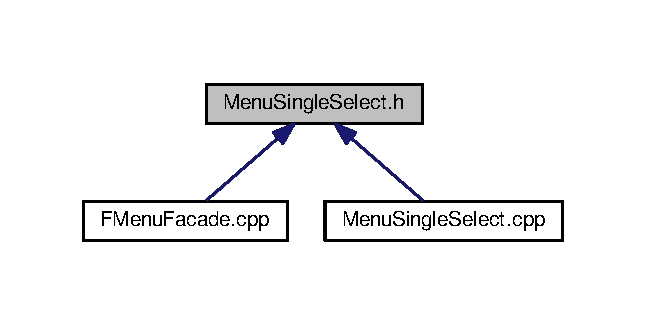
\includegraphics[width=310pt]{MenuSingleSelect_8h__dep__incl}
\end{center}
\end{figure}
\subsection*{Classes}
\begin{DoxyCompactItemize}
\item 
class \hyperlink{classMenuSingleSelect}{Menu\+Single\+Select}
\end{DoxyCompactItemize}

\hypertarget{RemoveVisitor_8cpp}{}\section{Remove\+Visitor.\+cpp File Reference}
\label{RemoveVisitor_8cpp}\index{Remove\+Visitor.\+cpp@{Remove\+Visitor.\+cpp}}
{\ttfamily \#include \char`\"{}Remove\+Visitor.\+h\char`\"{}}\\*
{\ttfamily \#include \char`\"{}Menu\+Multi\+Select.\+h\char`\"{}}\\*
Include dependency graph for Remove\+Visitor.\+cpp\+:
\nopagebreak
\begin{figure}[H]
\begin{center}
\leavevmode
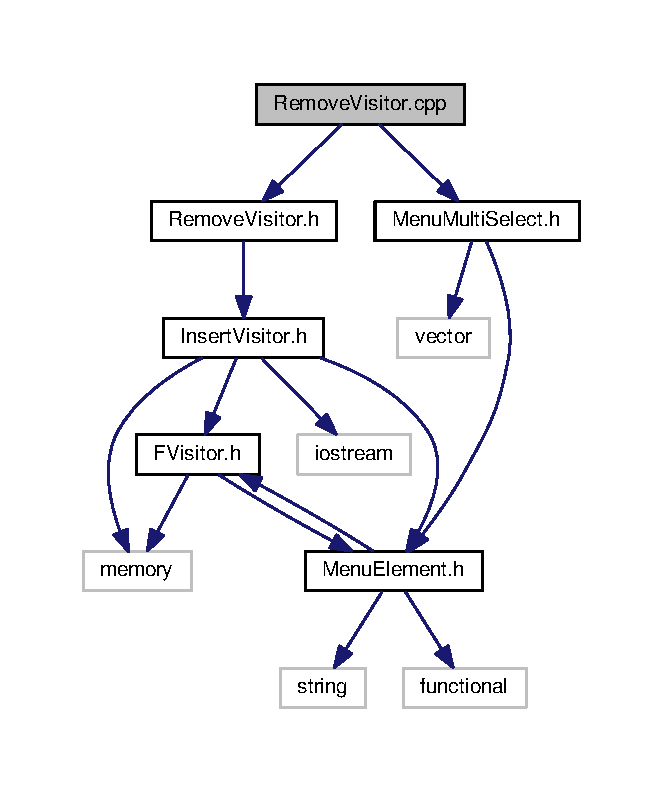
\includegraphics[width=318pt]{RemoveVisitor_8cpp__incl}
\end{center}
\end{figure}

\hypertarget{RemoveVisitor_8h}{}\section{Remove\+Visitor.\+h File Reference}
\label{RemoveVisitor_8h}\index{Remove\+Visitor.\+h@{Remove\+Visitor.\+h}}
{\ttfamily \#include \char`\"{}Insert\+Visitor.\+h\char`\"{}}\\*
Include dependency graph for Remove\+Visitor.\+h\+:
\nopagebreak
\begin{figure}[H]
\begin{center}
\leavevmode
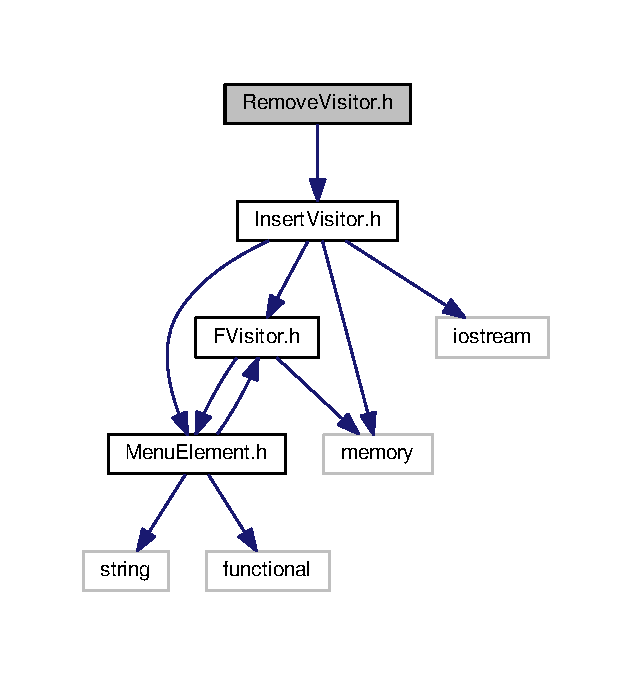
\includegraphics[width=304pt]{RemoveVisitor_8h__incl}
\end{center}
\end{figure}
This graph shows which files directly or indirectly include this file\+:
\nopagebreak
\begin{figure}[H]
\begin{center}
\leavevmode
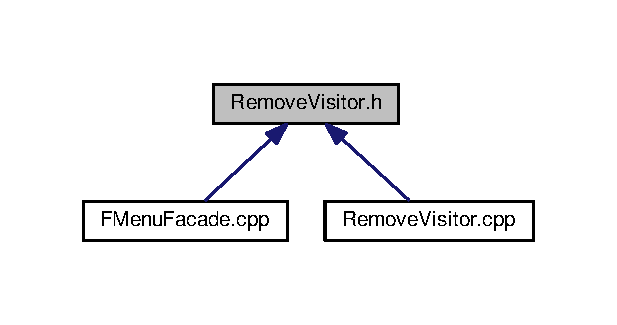
\includegraphics[width=296pt]{RemoveVisitor_8h__dep__incl}
\end{center}
\end{figure}
\subsection*{Classes}
\begin{DoxyCompactItemize}
\item 
class \hyperlink{classRemoveVisitor}{Remove\+Visitor}
\end{DoxyCompactItemize}

\hypertarget{SelectElementVisitor_8cpp}{}\section{Select\+Element\+Visitor.\+cpp File Reference}
\label{SelectElementVisitor_8cpp}\index{Select\+Element\+Visitor.\+cpp@{Select\+Element\+Visitor.\+cpp}}
{\ttfamily \#include \char`\"{}Select\+Element\+Visitor.\+h\char`\"{}}\\*
Include dependency graph for Select\+Element\+Visitor.\+cpp\+:
\nopagebreak
\begin{figure}[H]
\begin{center}
\leavevmode
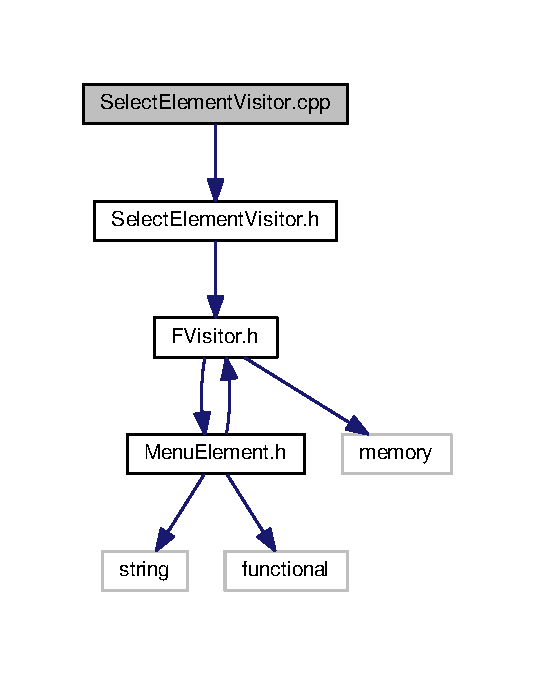
\includegraphics[width=257pt]{SelectElementVisitor_8cpp__incl}
\end{center}
\end{figure}

\hypertarget{SelectElementVisitor_8h}{}\section{Select\+Element\+Visitor.\+h File Reference}
\label{SelectElementVisitor_8h}\index{Select\+Element\+Visitor.\+h@{Select\+Element\+Visitor.\+h}}
{\ttfamily \#include \char`\"{}F\+Visitor.\+h\char`\"{}}\\*
Include dependency graph for Select\+Element\+Visitor.\+h\+:
\nopagebreak
\begin{figure}[H]
\begin{center}
\leavevmode
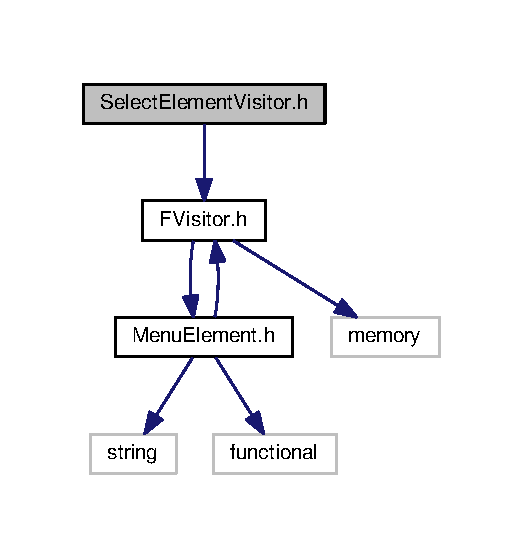
\includegraphics[width=251pt]{SelectElementVisitor_8h__incl}
\end{center}
\end{figure}
This graph shows which files directly or indirectly include this file\+:
\nopagebreak
\begin{figure}[H]
\begin{center}
\leavevmode
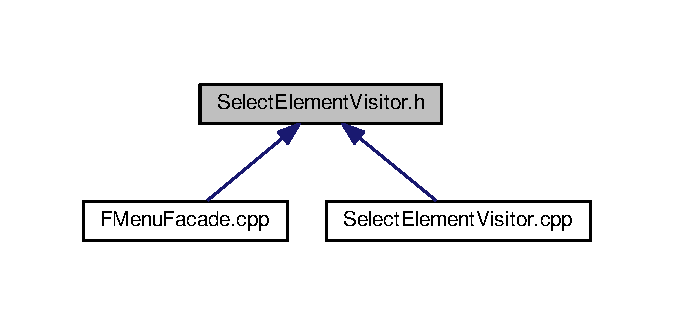
\includegraphics[width=324pt]{SelectElementVisitor_8h__dep__incl}
\end{center}
\end{figure}
\subsection*{Classes}
\begin{DoxyCompactItemize}
\item 
class \hyperlink{classSelectElementVisitor}{Select\+Element\+Visitor}
\end{DoxyCompactItemize}

%--- End generated contents ---

% Index
\backmatter
\newpage
\phantomsection
\clearemptydoublepage
\addcontentsline{toc}{chapter}{Index}
\printindex

\end{document}
